%% Use [handout] option for removing pauses
\documentclass[presentation,12pt]{beamer} 

\usepackage{etex}
% \usepackage[cp1251]{inputenc}
% \usepackage[T2A]{fontenc}
\usepackage[english]{babel}
\usepackage{amsmath}
\usepackage{amssymb}
\usepackage{amstext}
\usepackage{mathtools}
\usepackage{bbm} % For indicator function
\usepackage{color}
\usepackage{xcolor}
\usepackage{mathrsfs}
\usepackage{longtable}
\usepackage{geometry}
\usepackage{setspace}
\usepackage{graphicx}
\usepackage{multicol}
\usepackage{caption}
\usepackage{pgfplots}
\usetikzlibrary{shapes,fit, calc} % For fitting rectangles in pictures
\usepackage{array}
\usepackage{bookman}
\usepackage{booktabs}
\usepackage{appendixnumberbeamer}
\usepackage[absolute,overlay]{textpos}

\pgfplotsset{compat=1.8}

\title{Statistical Mechanics \\ and Information Theory \\ in Approximate Robust Inference \\[10pt] \hrule}
\author[Alexey~Gronskiy]
{ %
\footnotesize%
Doctoral Examination \\
%
Candidate: Alexey Gronskiy\\[8pt]
%
Examination Committee: \\
Prof. Dr. Joachim M. Buhmann \\
Prof. Dr. Peter Widmayer \\
Prof. Dr. Wojciech Szpankowski \\[8pt]
%
Chair: Prof. Dr. Onur Mutlu \\[-.5cm]
}

% \institute % (optional, but mostly needed)
% {
%   \inst{1}%
%   ETH Zurich, \{jbuhmann, alexeygr\}@inf.ethz.ch, julien.dumazert@gmail.com, 
%   \and
%   \inst{2}%
%   Purdue University, spa@cs.purdue.edu
% }
  
\date[ETH Zurich, D-INFK, 6 Mar 2018]{{\scriptsize ETH Zurich, D-INFK \qquad 6th March 2018}}

% \title{Statistical Mechanics \\ and Information Theory \\ in Approximate Robust Inference \\[10pt] \hrule}
% \author[Alexey~Gronskiy]
% { \footnotesize 
%    PhD Examination of Alexey Gronskiy \\[2pt]

   
% }

% % \institute % (optional, but mostly needed)
% % {
% %   \inst{1}%
% %   ETH Zurich, alexeygr@inf.ethz.ch
% % }
  
% \date[ETH Zurich, 6 Mar 2018]{{\small ETH Zurich \\ 6th March 2018}}

\usetheme{default}
\usecolortheme{default}
\useoutertheme{umbcfootline}
\usefonttheme{professionalfonts}
\definecolor{light-gray}{gray}{0.75}
\setbeamercolor{block body}{bg=gray!20}

\setfootline{
  \textcolor{gray!60}{
    \tiny\insertshortdate \hfill \insertshortauthor \quad 
    \insertframenumber/\inserttotalframenumber
  }
}

\newcommand{\setroadmapfootline}{%
\setfootline{%
  \textcolor{gray!60}{%
    \tiny\insertshortdate \hfill \insertshortauthor \quad 
    \phantom{\insertframenumber/\inserttotalframenumber}
  }%
}%
}

% \renewcommand\mathfamilydefault{\sfdefault} 
\renewcommand\familydefault{\sfdefault}

% \setbeamercovered{transparent}
\beamertemplatenavigationsymbolsempty

\setbeamertemplate{itemize items}[circle]
\setbeamertemplate{frametitle}[default][center]
% \setbeamertemplate{frametitle}{\centering\insertframetitle\par\vskip-6pt\hrulefill}

\captionsetup{figurename=}

% Useful macros
\newcommand{\vect}[1]{\boldsymbol{\mathbf{#1}}}

\newcommand{\Expct}{\mathbb{E}}
\newcommand{\Var}{\mathrm{Var}}
\newcommand{\Cov}{\mathrm{Cov}}
\newcommand{\Ind}{\mathbbm{1}}
\newcommand{\Prob}{\mathbb{P}}
\def\D{{\cal D}}
\def\C{{\cal C}}
\def\S{{\cal S}}
\def\X{{\cal X}}
\def\H{{\cal H}}
\def\E{{\mathbb E}}

\newcommand{\todo}{\textbf{\colorbox{red}{TODO}}}

% ===========================
\begin{document}

%% Title page without footline
{
\setbeamertemplate{footline}{} 
\begin{frame}[noframenumbering]
  \titlepage
\end{frame}
}

{\setroadmapfootline \begin{frame}[noframenumbering]{Roadmap}
\centering
\includegraphics[width=\textwidth]{roadmap_start} 
\end{frame}}

{\setroadmapfootline \begin{frame}[noframenumbering]{Regularizing by Gibbs Algorithm}
\centering
\includegraphics[width=\textwidth]{roadmap_after_start} 
\end{frame}}

% \begin{frame}{Generic Problem}
% \begin{center}
%   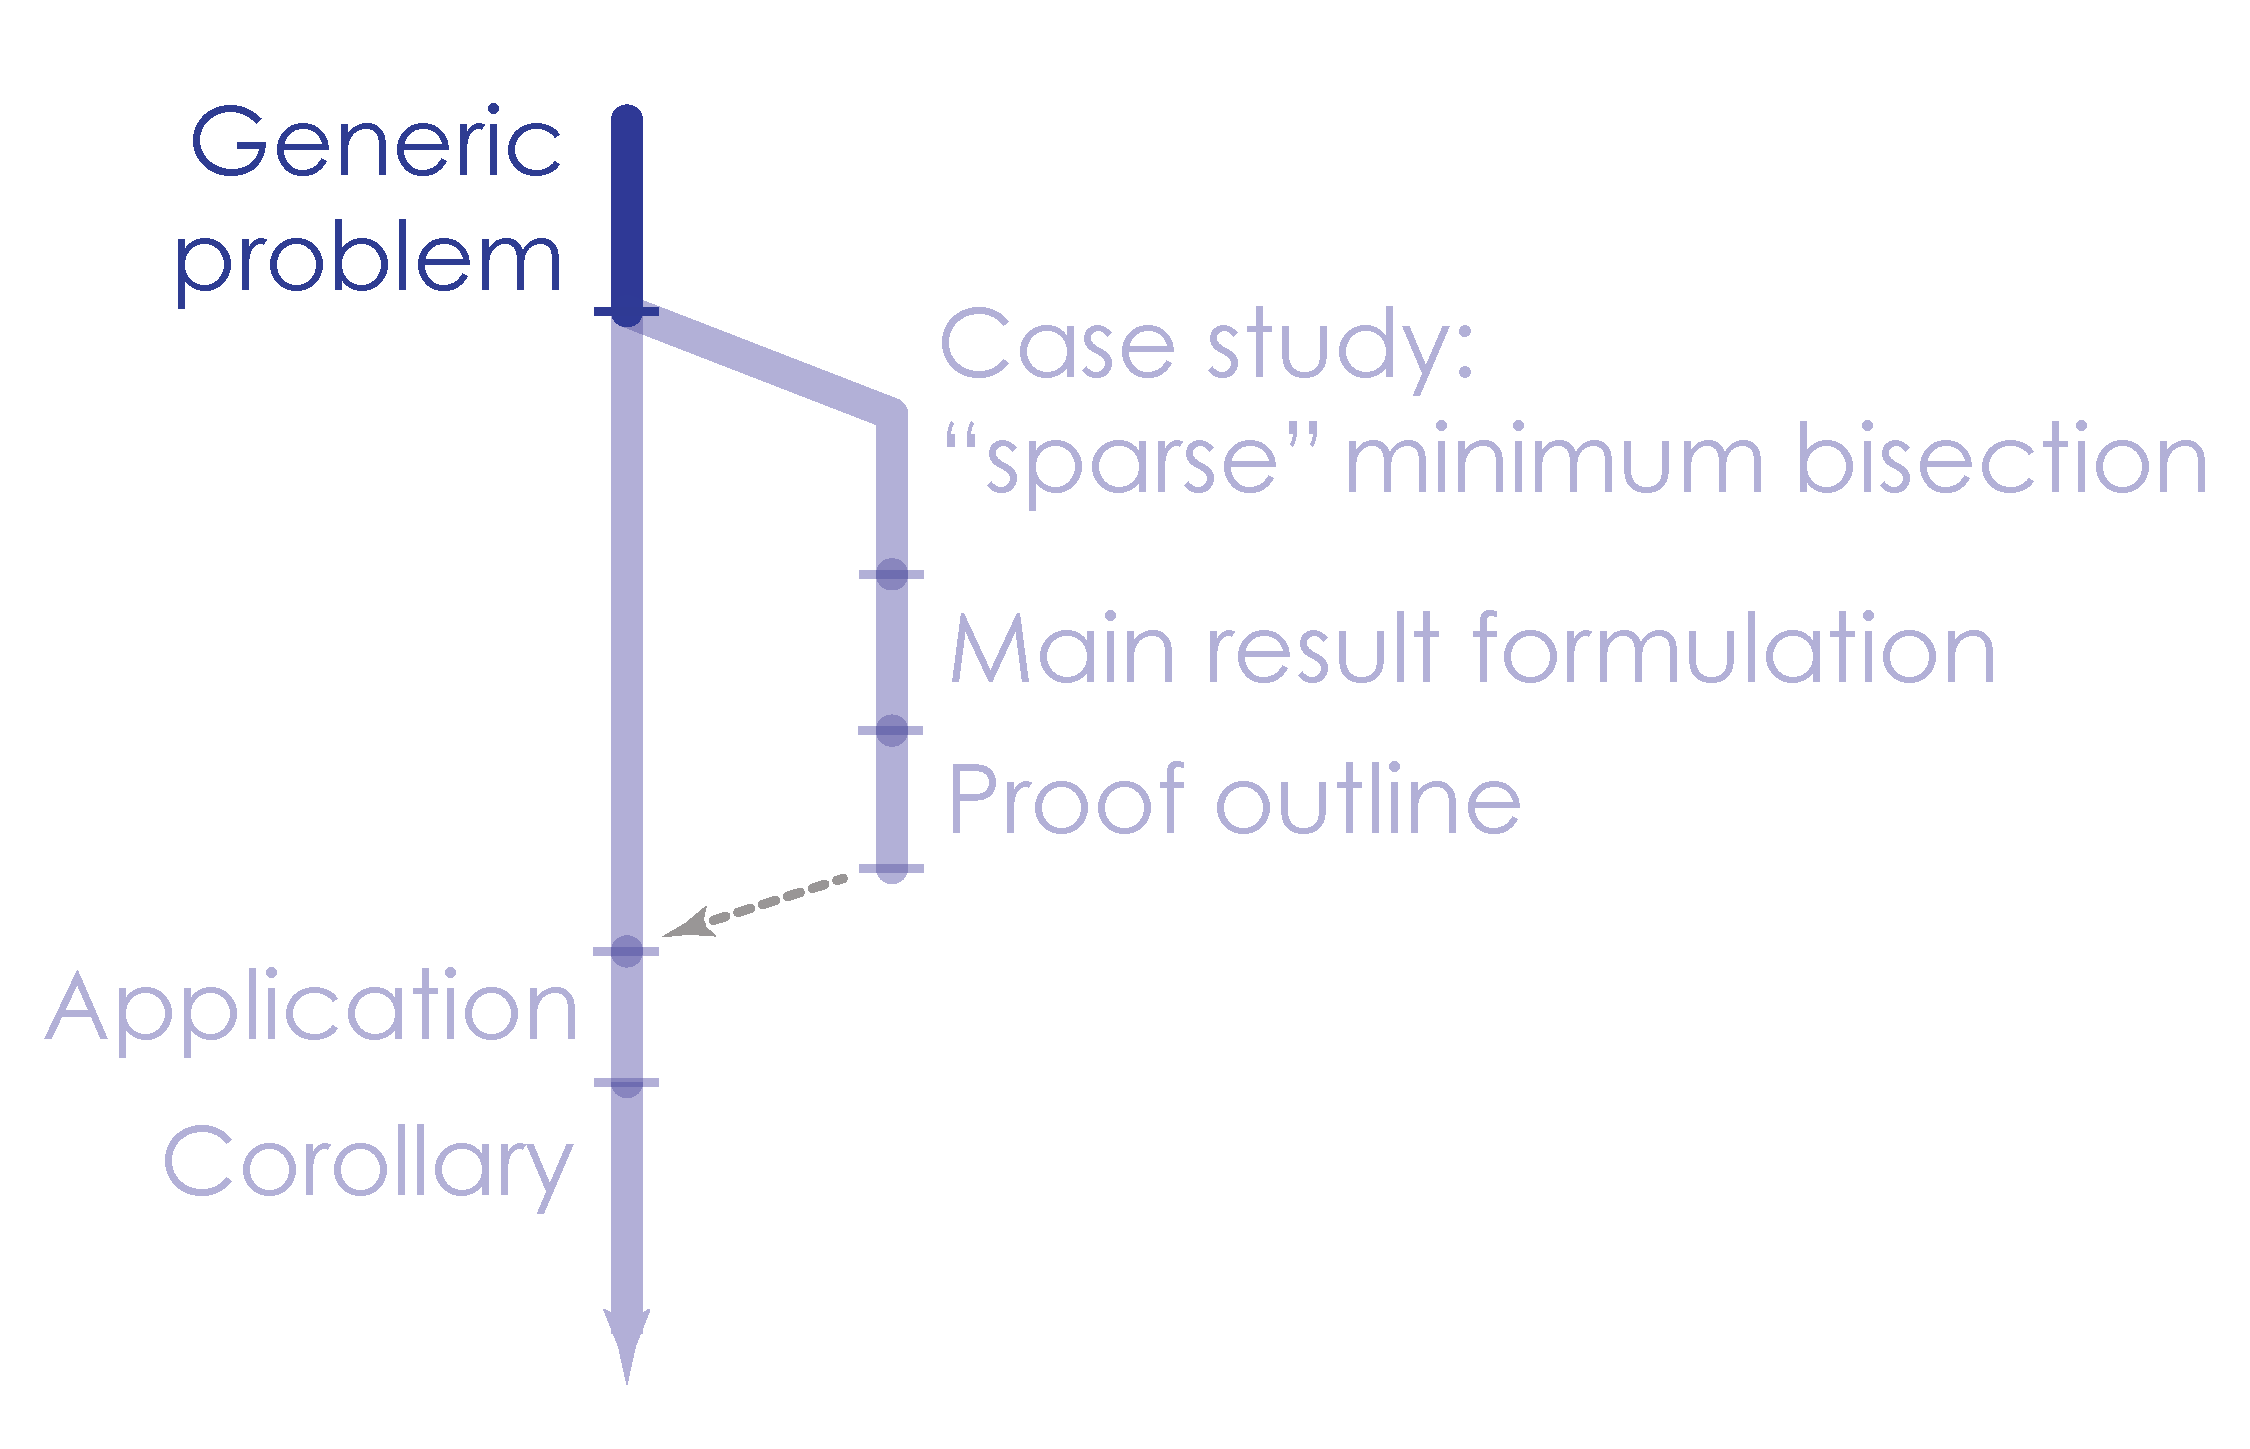
\includegraphics[scale=.27]{GenericProblem.pdf} 
% \end{center}
% \end{frame}

\begin{frame}{Generic Optimization Problem}
  
  As a motivation, we bring up a generic randomized optimization problem, where \\[2pt]
  \begin{itemize}
  \item $X \in \X$ random data instance $X$ as an element of set $\X$ \\[.4cm]
  \item $c \in \C$ is solution $c$ as element of solution set $\C$ \\[.4cm]
  \item $R(c, X)$ is cost function of solution $c$ given in a data instance $X$
  \end{itemize}

\end{frame}

\begin{frame}{Regularizing by Gibbs Algorithm}
\begin{itemize}
  \item<+-> Recall possible standard approach (ERM):

  \begin{center}
    \hspace{-8mm}\includegraphics[scale=.4]{standard-erm-explanation} 
  \end{center}
  
  % \textbf{Regularizer} is a part of $R(c, X)$ \\[.5cm]

  \item<+-> The approach we focus on:

  \begin{center}
    \hspace{-8mm}\includegraphics[scale=.4]{posterior-distribution-explanation} 
  \end{center}
  
  \textbf{Regularizer} is inverse temperature $\beta$~--- controls ``width''

\end{itemize}
\end{frame}

\begin{frame}{Regularizing by Gibbs Algorithm}
\begin{columns}[T]
    \begin{column}{0.6\textwidth}
    \begin{itemize}
    \setlength\itemsep{1em}
    \item<+-> We search for stochastic approximation: 
    \[
      X \longmapsto c \sim p(c|X)
    \]
    \item<+-> Define a \textbf{Gibbs posterior} over solutions: \\
    \vspace*{6pt} 
    \hspace{5em} $\Downarrow$ 
    \[
      p_\beta(c|X) \propto \exp( - \beta \cdot R(c,X))
    \]
  \end{itemize}
  \end{column}

    \begin{column}{0.4\textwidth}
      \onslide<2>{
        \includegraphics[width=\textwidth]{gibbs_example.eps}
      }
    \end{column}

\end{columns}
\end{frame}

\begin{frame}{Motivation for Gibbs Distribution}
  \begin{itemize}
  \item Represents the family of \textbf{maximum entropy} [1] distributions for the fixed
  expected costs:
    \[
        p_\beta(c|X) \in \arg \max_{\substack{p(c|X) \colon \\ \Expct[R(c, X)] = r}} H(p)
    \]

  \item Minimizes the expected risk, \textbf{regularized} by the input-output mutual
  information [2]:
    \[
        p_\beta(c|X) \in \arg \min_{p(c|X)} \Bigl( \Expct[R(c, X)] +
          \frac{1}{\beta} I(c, X) \Bigr)
    \]
  \end{itemize}

  \vfill

  {
  \setstretch{0.7}
  \textcolor{gray!60}{
    \scriptsize [1] Jaynes (1957), \textit{Information Theory and Statistical Mechanics},
    \\ Phys. Review, Ser. II }\par

  \textcolor{gray!60}{
    \scriptsize [2] Xu and Raginsky (2017), 
    \textit{Information-theoretic analysis of generalization capability of
      learning algorithms}, NIPS 2017 }\par
  }
\end{frame}

{\setroadmapfootline \begin{frame}[noframenumbering]{Large Disordered Systems}
\centering
\includegraphics[width=\textwidth]{roadmap_after_gibbs} 
\end{frame}}

\begin{frame}{Free Energy}

Now 
\[ p(c|X) = \exp \bigl( -\beta \cdot R(c,X) - \mathcal{F}(X) \bigr), \]

\medskip
where the following is \textbf{Helmholtz free energy}:
\[\mathcal{F}(\beta, X) = \log Z(\beta, X), \]
here $Z(\beta, X)$ is \textbf{partition function}:
\[
\quad Z(\beta, X) = \sum_{c'\in \C} \exp(-\beta R(c', X))
\]

\medskip

\uncover<2->{\textcolor{green!50!black}{\textbf{Issue:}} Understanding the stochastic behavior of $\log
Z(\beta, X)$ is known to be \textbf{hard}.}
        
\end{frame}

\begin{frame}{Statistical Mechanics of Free Energy}

  \begin{itemize}
    \item Empirical quantity:  $\log Z(\beta, X)$
    \item \textbf{Annealed} average (easy but ``wrong''):  \\
      \[ \mathcal{F}(\beta, X) = \log {\color{red} \Expct_X} [Z(\beta, X)]  \]
    \item \textbf{Quenched} average (hard but ``correct''):   \\
     \[ \mathcal{F}(\beta, X) = {\color{green!50!black} \Expct_X} \bigl[\log Z(\beta, X)\bigr] \]
  \end{itemize}

  \bigskip
  \textbf{Our goal} is to \textbf{asymptotically} study its quenched
      approximation. 
      \[
        \boldsymbol{\lim_{\text{size} \to \infty} \Expct_X \log Z(\beta, X) = \; ?}
      \]
\end{frame}

{\setroadmapfootline \begin{frame}[noframenumbering]{``In Vitro'' Combinatorial Problem}
\centering
\includegraphics[width=\textwidth]{roadmap_after_free_energy} 
\end{frame}}

\begin{frame}{``In Vitro'' Combinatorial Problem: \\ ``Sparse'' Minimum Bisection -- I}
\begin{itemize}
  \item<+-> \textbf{Given:} complete graph with random edge weights
    \[G = (V, E, X), \quad X = \{W_i\}_{i \in E}\]
  \item<+-> \textbf{Find:} two subgraphs 
    \[c = (U_1, U_2), \quad U_1 \sqcup U_2 \subsetneq V \]
  of a small size $d$ (``sparsity'')  
  \item<+-> Such that the \textbf{total edge cost} between them is minimal
    \[ \arg \min_{c = (U_1, U_2)} R(c, X) = \arg \min_{c = (U_1, U_2)} \sum_{i \in \mathrm{edges}(c)} W_i \]
\end{itemize}
\end{frame}

\begin{frame}{``In Vitro'' Combinatorial Problem: \\ ``Sparse'' Minimum Bisection -- II}
\only<1>{
  \begin{center}\includegraphics[width=.8\textwidth]{smbp_illustration.eps}\end{center}
}

\only<2>{
  \begin{center}\includegraphics[width=.6\textwidth]{smbp_illustration.eps}\end{center}
  \[
        \boldsymbol{\lim_{n \to \infty} \Expct_X \log Z(\beta, X) = \; ?}
  \]
}
\end{frame}

\begin{frame}{Free Energy: Short Overview -- I}

  \begin{itemize}
    \item Notorious difficulty of computing $\Expct \log Z$ is related [1][2]
      to dependencies in solutions: 
      \[\Cov(R(c', X), R(c'', X)) \ne 0.\]

    \item %
      \begin{minipage}[t]{0.5\linewidth}
        In our case, the dependencies \textbf{exist} but are \textbf{small}.
      \end{minipage}%
      \begin{minipage}[t]{0.5\linewidth}%
        \centering %
        \vspace{-4pt}\includegraphics[width=.7\textwidth]{different_solution_overlaps_3}
      \end{minipage}   
    
    \item Large correlations require additional work (conjecture in appendix). 
  \end{itemize}

  {
    \setstretch{0.7}
    \textcolor{gray!60}{
      \scriptsize [1] Bovier (2012), 
      \textit{Statistical Mechanics of Disordered Systems: A Mathematical Perspective}, Cambridge 
    }\par

    \textcolor{gray!60}{
      \scriptsize [2] Talagrand (2003), 
      \textit{Spin Glasses: A Challenge for Mathematicians}, Springer 
    }\par
  }
\end{frame}

\begin{frame}{Free Energy: Short Overview -- II}

\begin{itemize}
  \item Derrida [1] established Random Energy Model~--- a model where solution costs are independent;
  \[
    \lim_{n\to \infty} \frac{\E[\log Z(\beta, X)]}{n}=
    \left\{ \begin{array}{ll}
    \frac{\beta^2}{4}+\log 2 & 
    \beta < 2 \sqrt{\log 2},\\
    \beta \sqrt{\log 2} & \beta \ge 2 \sqrt{\log 2}.
    \end{array}
    \right.
  \]
  
  \item Vannimenus and M\'ezard [2] solved free energy for Traveling Salesman
    Problem: \textbf{small dependencies}.
  
  \bigskip

  % \item<+-> \textbf{[Talagrand'02]}:
  %   systematization; simple proof of REM free energy phase transition and beyond:
  %   \[
  %     \lim_{n\to \infty} \frac{\E[\log Z(\beta, X)]}{n}=
  %     \left\{ \begin{array}{ll}
  %     \frac{\beta^2}{4}+\log 2 & 
  %     \beta < 2 \sqrt{\log 2},\\
  %     \beta \sqrt{\log 2} & \beta \ge 2 \sqrt{\log 2}.
  %     \end{array}
  %     \right.
  %   \]
\end{itemize}

\vfill

{
  \setstretch{0.7}
  \textcolor{gray!60}{
    \scriptsize [1] Derrida (1981), 
    \textit{Random-energy model: An exactly solvable model of disordered systems},
    Phys. Rev. B 24} \\
  \textcolor{gray!60}{
    \scriptsize [2] Vannimenus and M\'ezard (1984), 
    \textit{On the Statistical Mechanics of Optimization Problems of the traveling Salesman Type}, 
    J. de Physique Lettres, 45, 1984} \par
}

\end{frame}

{\setroadmapfootline \begin{frame}[noframenumbering]{Main Result}
\centering
\includegraphics[width=\textwidth]{roadmap_after_in_vitro} 
\end{frame}}
% \begin{frame}{Our Results}

% \begin{frame}

% \begin{frame}{Conclusions}

% \end{frame}

% \begin{frame}{Notation}
  
%   \begin{table}[!ht]
%   %\makebox[\textwidth][c]{%
%   \footnotesize\renewcommand{\arraystretch}{1.4}%
%   \begin{tabular}{@{}lll@{}}
%           \toprule
%           Notation & Meaning \tabularnewline \midrule 
%           $X \in \X$ & Dataset $X$ (instance) as an element of a dataset space $\X$\\
%           $c \in \C$ & Solution $c$ as element of solution set $\C$ for a given problem \\
%           $R(c, X)$ & Cost function of solution $c$ given a data instance $X$ \\
%           $p_\beta(c|X)$ & Posterior probability of solution given data at resolution $\beta$\\
%           $\H(\ldots)$ & Entropy of a random variable \\
%   \bottomrule
%   \end{tabular}%
%   %}
%   \end{table}
% \end{frame}

% \begin{frame}{Maximum Entropy Inference\\ in Machine Learning}
% \begin{itemize}
% \item<+-> Learning and Inference: given \textbf{noisy data} $X$, provide a \textbf{robust solution} $c$.
% \item<+-> Maximum Entropy principle: find a \emph{maximally non-committal} posterior
%   distribution \uncover<+->{"with regard to missing information" [Jaynes'57].}
% \item<+-> Inference by the Maximum Entropy principle 
% %(not the only one!)
% %%%JB Alex, here you should state the alternatives, but I find this
% %%% not very enlightening at this point of the talk. 
%   results in the \textbf{Gibbs posterior distribution}
%   \[
%         \alert<-.>{p_\beta(c | X)} =\frac{\exp\bigl(-\beta R(c, X)\bigr)
%         }{ \sum_{\tilde{c}\in \C} \exp\bigl(-\beta R(\tilde{c}, X)\bigr) },
%   \]
%   which puts the higher weights on more optimal solutions.
% \item<+-> Examples of Gibbs distributions: Gaussian, Exponential and many others...
% \end{itemize}
% \end{frame}

% \begin{frame}{Physical Interpretation}
% \begin{itemize}
% \item<+-> {}[Vannimenus, M\'ezard '84] ``On the statistical mechanics of optimization problems of the travelling salesman type''.
% \item<+-> Every solution
%   specifies a \textbf{configuration} $c \in \C$; cost function $R(c,
%   X)$ defines 
%   \textbf{energy (Hamiltonian)} of the configuration; the quantity $\beta$ denotes
%   \textbf{inverse temperature}.
% \item<+-> ``Natural'' limiting behavior of Gibbs distribution: 
% \begin{columns}[T]
%     \begin{column}{0.5\textwidth}
%     \centering
%      \[
%       \qquad\lim_{\alert<4>{\beta \to \only<-3>{0}\only<4>{\infty}}} p_\beta(c | X) =
%     \begin{overprint}
%     \only<3>{\frac{1}{|\C|}}%
%      \only<4>{\frac{\mathbb{I}\{c \in \C_0\}}{|\C_0|}}
%     \end{overprint}
%       \]
%        \only<4>{$\C_0$ are optimal solutions.}
%     \end{column}
%     \begin{column}{0.5\textwidth}
%       \begin{tikzpicture}
\begin{axis}[
	footnotesize,
	width=\textwidth,
	xticklabels={,,},
	yticklabels={,,},
	ymin=0,
    	ymax=0.5,
	xlabel=configurations,
	ylabel=posteriors
	]
\only<3>{\addplot+[const plot mark mid]
coordinates
{ (0.1,0.1)  (0.2,0.1)   (0.3,0.1)
 (0.4,0.1) (0.5,0.1)  (0.6,0.1)  (0.7,0.1)
 (0.8,0.1) (0.9,0.1)  (1,0.1)};}
 \only<4>{\addplot+[const plot mark mid]
coordinates
{ (0.1,0)  (0.2,0.33)   (0.3,0)
 (0.4,0) (0.5,0.33)  (0.6,0)  (0.7,0.33)
 (0.8,0) (0.9,0)  (1,0)};}
\end{axis}
\end{tikzpicture}
%     \end{column}
% \end{columns}
% \end{itemize}
% \end{frame}

% \begin{frame}{Posteriors for Two Instances}
% \begin{columns}
%     \begin{column}{0.6\textwidth}
%       \centering
%       \begin{tikzpicture}
	\begin{axis}[
	footnotesize,
	width=\textwidth,
	height=0.8\textheight,
	xticklabels={,,},
	yticklabels={,,},
	ymin=0,
    	ymax=1.5,
	xlabel=solutions,
	ylabel=Gibbs measures
	]
	% \only<1>{\addplot[
	%    red,
	%    domain=-2:2,
	%    samples=201,
	% ]
	%    {exp(-(x+0.25)^2 / (2*0.1)) / (sqrt(0.1 * 2*pi))};
	% \addplot[
	%    blue,
	%    domain=-2:2,
	%    samples=201,
	% ]
	%    {exp(-(x-0.25)^2 / (2*0.1)) / (sqrt(0.1 *2*pi))};
	%    \draw[densely dashed] ({axis cs:-0.25,0}|-{rel axis cs:0,0}) -- ({axis cs:-0.25,0}|-{rel axis cs:0,1});
	%    \draw[densely dashed] ({axis cs:0.25,0}|-{rel axis cs:0,0}) -- ({axis cs:0.25,0}|-{rel axis cs:0,1});}%
	% %%
	% \only<2>{\addplot[
	%    red,
	%    domain=-2:2,
	%    samples=201,
	% ]
	%    {exp(-(x+0.5)^2 / (2*0.1)) / (sqrt(0.1 * 2*pi))};
	% \addplot[
	%    blue,
	%    domain=-2:2,
	%    samples=201,
	% ]
	%    {exp(-(x-0.5)^2 / (2*0.1)) / (sqrt(0.1 *2*pi))};
	%    \draw[densely dashed] ({axis cs:-0.5,0}|-{rel axis cs:0,0}) -- ({axis cs:-0.5,0}|-{rel axis cs:0,1});
	%    \draw[densely dashed] ({axis cs:0.5,0}|-{rel axis cs:0,0}) -- ({axis cs:0.5,0}|-{rel axis cs:0,1});}%
	% %%
	% \only<3>{\addplot[
	%    red,
	%    domain=-2:2,
	%    samples=201,
	% ]
	%    {exp(-(x+1)^2 / (2*0.1)) / (sqrt(0.1 * 2*pi))};
	% \addplot[
	%    blue,
	%    domain=-2:2,
	%    samples=201,
	% ]
	%    {exp(-(x-1)^2 / (2*0.1)) / (sqrt(0.1 *2*pi))};}%
	% \only<3->{%
	% \draw[densely dashed] ({axis cs:-1,0}|-{rel axis cs:0,0}) -- ({axis cs:-1,0}|-{rel axis cs:0,1});
	% \draw[densely dashed] ({axis cs:1,0}|-{rel axis cs:0,0}) -- ({axis cs:1,0}|-{rel axis cs:0,1});}%
	%   %%
	\addplot[
	   red,
	   domain=-2:2,
	   samples=201,
	]
	   {exp(-(x+1)^2 / (2 * 0.5)) / (sqrt(0.3 * 2 * pi))};
	\addplot[
	   blue,
	   domain=-2:2,
	   samples=201,
	]
	   {exp(-(x-1)^2 / (2 * 0.5)) / (sqrt(0.3 * 2 * pi))};%
	% %%
	% \only<5->{\addplot[
	%    red,
	%    domain=-2:2,
	%    samples=201,
	% ]
	%    {exp(-(x+1)^2 / (2* 2)) / (sqrt(2 * 2 * pi))};
	% \addplot[
	%    blue,
	%    domain=-2:2,
	%    samples=201,
	% ]
	%    {exp(-(x-1)^2 / (2* 2)) / (sqrt(2 * 2 * pi))};}
	\end{axis}
	\end{tikzpicture}%
%     \end{column}
%     \begin{column}{0.4\textwidth}
%   The Gibbs posteriors for two noisy data instances \emph{could} look like that. \uncover<2->{\alert<-3>{Variance in noise can be the case!}}

%   Temperature:\\
%   \only<1-3>{high $\beta$}
%   \only<4>{\alert{decreasing $\beta$}}
%   \only<5->{\alert{low $\beta$}}
  
%   \medskip
%   \uncover<5->{This behavior explains why we prefer the high-temperature \alert{(low $\beta$)} limits for very noisy problems.}
%     \end{column}
% \end{columns}
% \end{frame}

% \begin{frame}{Posterior Agreement $\E_{X', X''} [I_\beta(X', X'')]$}
% \begin{itemize}
%   \item<+-> Thus $\beta$ is resolution parameter. \textbf{Q:} which $\beta$ to use for good noise adaptation?
%    \item<+-> {}[Buhmann'10, '11] Computing
%         expected posterior agreement for two instances $X'$, $X''$
%   \[
%           \E_{X', X''} [\alert<.>{I_\beta(X', X'')}] = \E \Bigl[ |\C| \log
%           \sum_{c \in \C} p_\beta(c | X') p_\beta(c | X'') \Bigr]
%   \]
%   \item<+-> ... has information-theoretic roots [Buhmann'10, '13];
% % \item<+-> ... defines a solution induced similarity \textbf{kernel between} instances
% % \[
% %   k(X', X'') := \sum_{c \in \C} p_\beta(c | X') p_\beta(c | X'') \in [0,1];
% % \]
%       \item<+-> \alert{... contains the partition function and the free energy~--- it is
%         worth understanding its behaviour.}
% \end{itemize}
% \end{frame}

% \begin{frame}{Free Energy and its Self-importance}
%   \begin{itemize}
%   \item<+-> The quantity
%     \[
%     -\frac{1}{\beta} \alert<3>{\log Z(\beta, X)} = -\frac{1}{\beta}
%      \alert<3>{\log \sum_{c\in \C} \exp\bigl(-\beta R(c, X)\bigr)}
%     \]
%     is called \textbf{free energy} and is one of the most important
%     properties of a system;
%   \item<+-> Why does $Z(\beta, X)$ matter? Consider conditional entropy:
%     \begin{align*}
%       \H(c\vert X) &= -\E_X \sum_{c\in \C} p_\beta(c | X) \log p_\beta(c | X) \\
% %      &= \E_X \log Z(\beta, X) - \E_X \sum_{c \in \C} \frac{- \beta
% %        R(c, X) e^{-\beta R(c, X)}}{Z(\beta, X)} \\
%       &= \E_X\alert<3>{ \log Z(\beta, X)} - \beta \frac{\partial
%         \E_X\alert<3>{\log Z(\beta, X)}}{\partial \beta}.
%     \end{align*}
%   \end{itemize}
% \end{frame}

% \begin{frame}{Self-averaging and Random Energy Model (REM)}
%   \begin{itemize}
%         \item<+-> Understanding how $\log Z(\beta, X)$ behaves in
%           various limits is one of the interesting fundamental questions!
%         \item<+-> \textbf{Random Energy Model} [Derrida'80]: the Hamiltonians $R(c,X)$ are r.v.
%         \item<+-> We can study ([Bonomi, Lutton'84]) 
%           $\E_X \log Z(\beta, X)$, taken w.r.t. the randomness in
%           Hamiltonians $R(c,X)$ due to \alert{self-averaging}.
%   \end{itemize}
% \end{frame}

% \begin{frame}{Some History}
%   \onslide<+->{\begin{block}{[Vannimenus, M\'ezard '84]}
%   \begin{itemize}
%     \item For TSP-type problem: in the high-temperature limit, the annealed approximation $\log \E_X Z(\beta, X)$ works well for the quenched approximation $\E_X \log Z(\beta, X)$;
%     \item Also gave indication that this works for other temperature limits.
%   \end{itemize}
%   \end{block}}
  
%   \onslide<+->{\begin{block}{[Talagrand'02]}
%     For the REM model with Gaussian Hamiltonians the normalized (in some way $f(n)$) free energy exhibits (asymptotically in $n\to \infty$) a phase transition
%     \[
%       \lim_{n\to \infty} \frac{\E[\log Z(\beta, X)]}{f(n)}=
%       \left\{ \begin{array}{ll}
%       \frac{\beta^2}{4}+\log 2 & 
%       \beta < 2 \sqrt{\log 2},\\
%       \beta \sqrt{\log 2} & \beta \ge 2 \sqrt{\log 2}.
%       \end{array}
%       \right.
%     \]
%   \end{block}}
% \end{frame}

% \begin{frame}{Main Result}
% \begin{center}
%   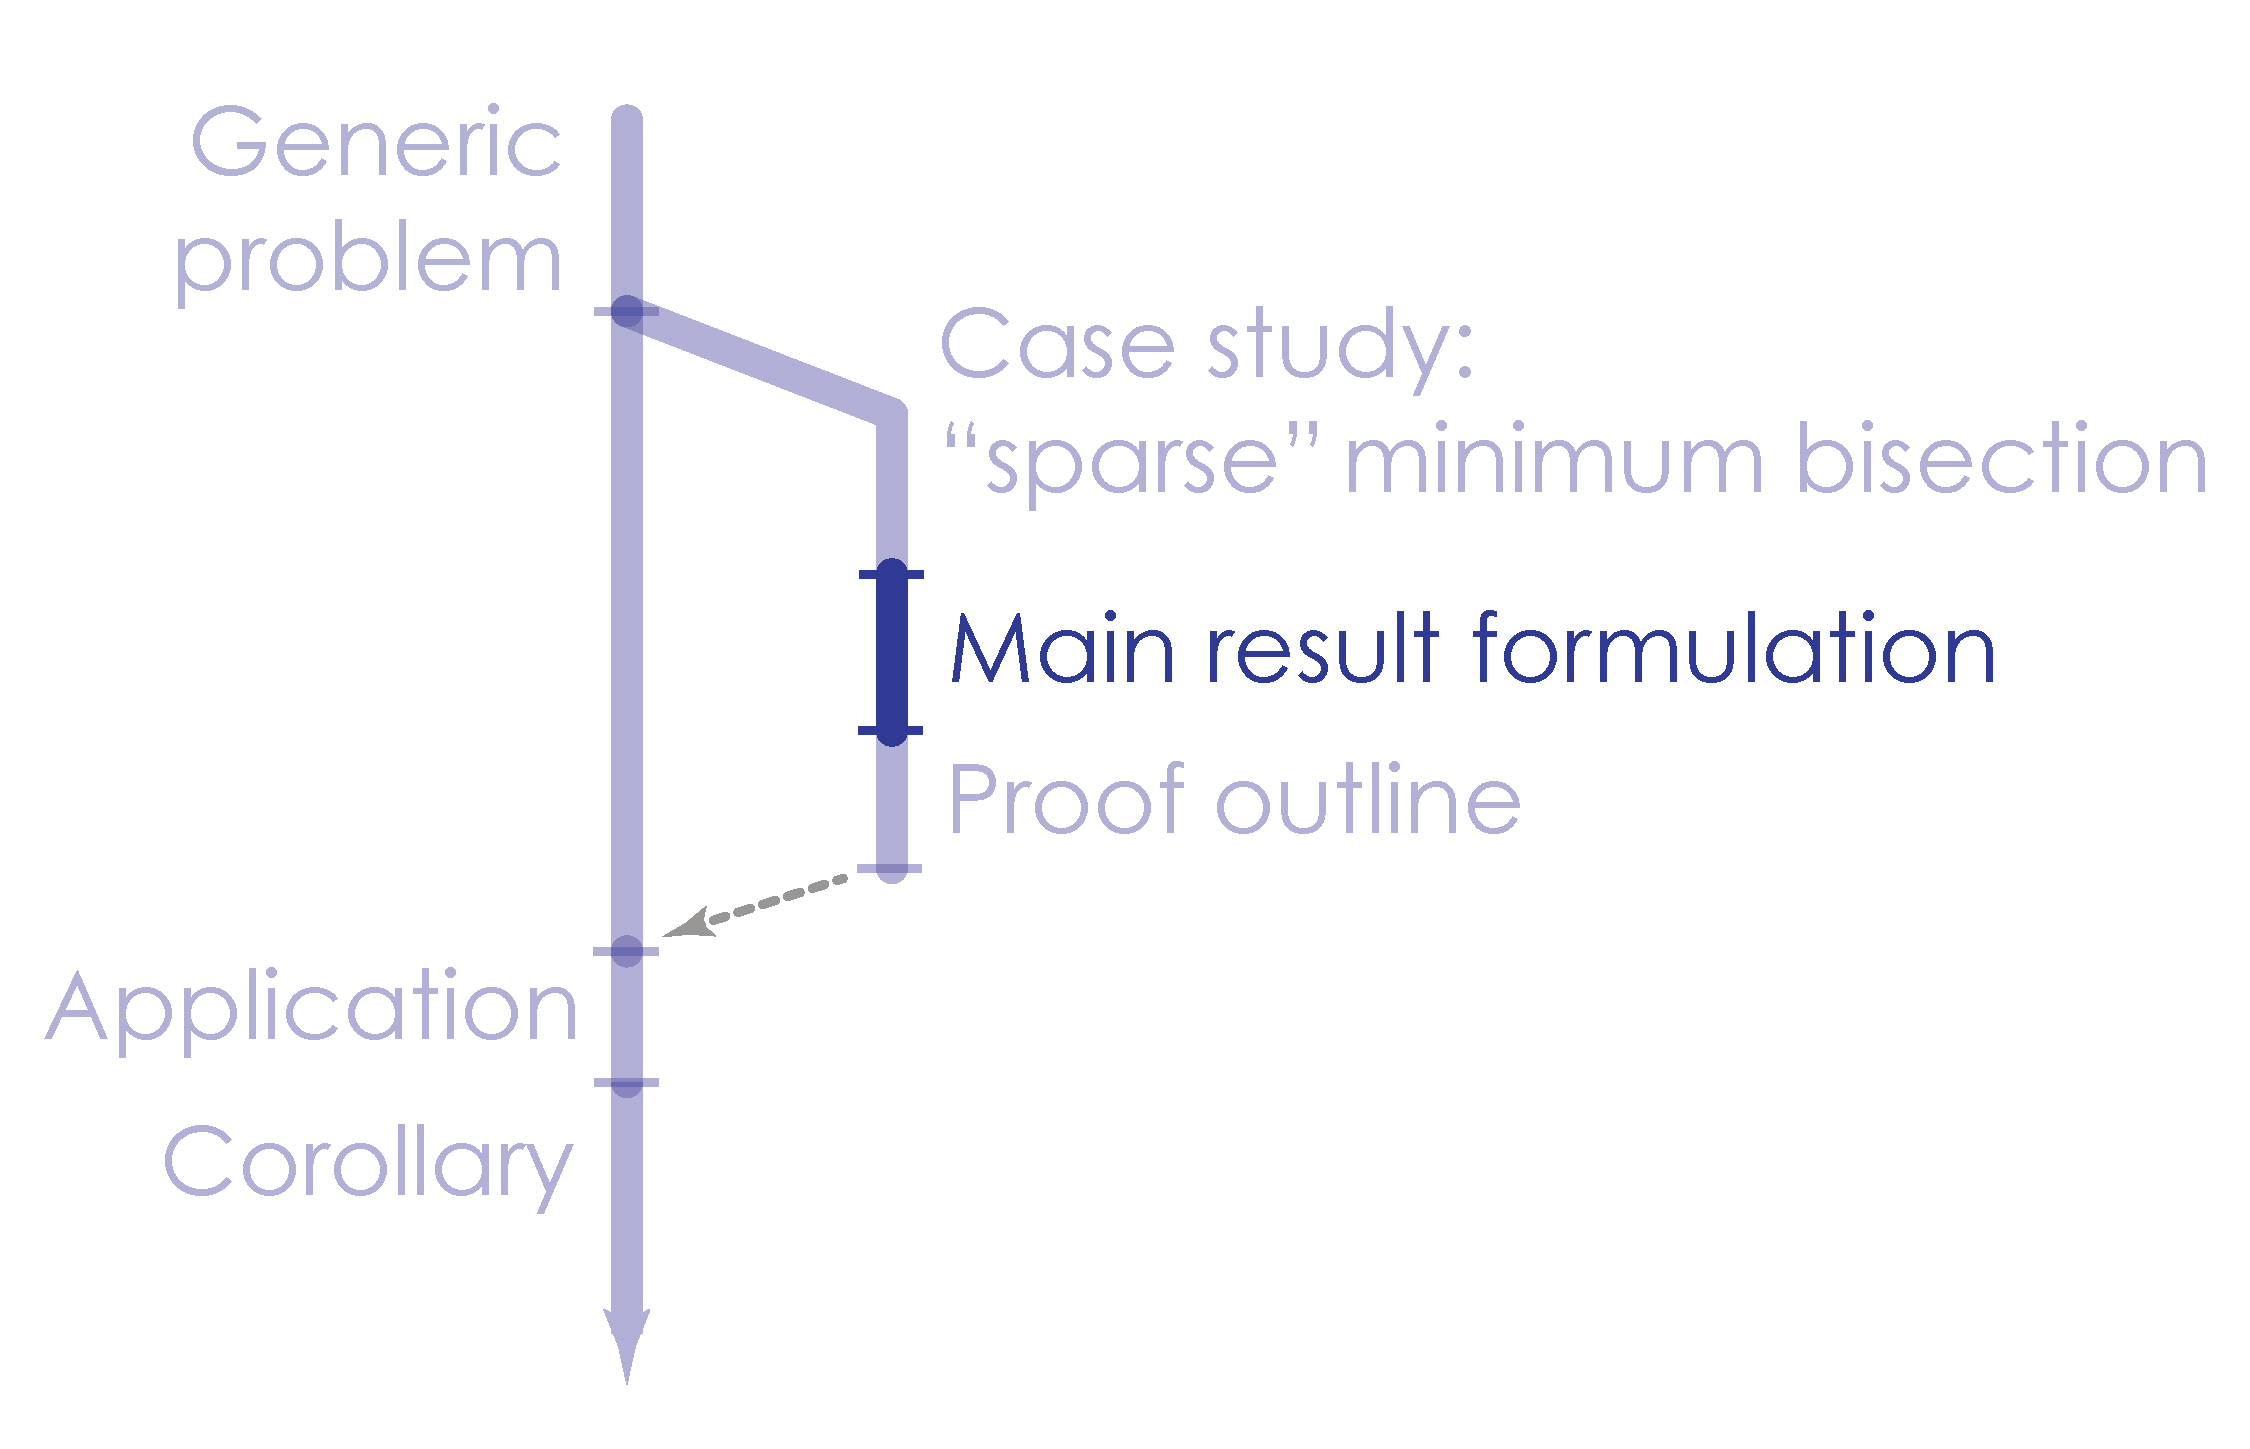
\includegraphics[scale=.27]{MainTheoremFormulation.pdf} 
% \end{center}

% \end{frame}

\begin{frame}{Main Result: Setting}
\begin{columns}[T]
\begin{column}{0.6\textwidth}
  \begin{itemize}
  \item<+-> $N$ is $\#$ of solution parameters:
  \[
    N \coloneqq |\mathrm{edges}(U_1, U_2)|
  \]
  \item<+-> $m$ is number of solutions:
  \[
    m \coloneqq |\C|
  \]
  \item<+-> require to be ``parameter rich'':
  \[
    \log m = o(N)
  \]
  \end{itemize}
\end{column}
\begin{column}{0.4\textwidth}
\centering \includegraphics[scale=.8]{smbp_notation}


\vfill
\hbox{}
\end{column}
\end{columns}
\end{frame}

\begin{frame}{Main Result}
\begin{block}{\rule[-0.6ex]{0pt}{2.5ex}Main theorem: free energy asymptotics}
  Assume:
  \begin{itemize}
    \item Sparse MBP on a complete graph
    \item Edge weights mutually independent
    within any given $c$
    \item Weights mean $\mu$ and variance $\sigma^2$, MGF $<\infty$
  \end{itemize}
  Then:
\[
\lim_{n\to \infty} \frac{\E[\log Z] +\hat \beta \mu \sqrt{N\log m}}{\log m} =
\left\{ \begin{array}{ll}
1+\frac{\hat \beta^2\sigma^2}{2}, &
\hat \beta< \frac{\sqrt{2}}{\sigma},\\
\hat \beta \sigma \sqrt{2}, & \hat \beta \ge \frac{\sqrt{2}}{\sigma}
\end{array}
\right.
\]
provided $\log n \ll d \ll \frac{n^{2/7}}{\sqrt{\log n}}$.

\end{block}
\end{frame}

% \begin{frame}{Proof: Bird's-eye View} 
%   \begin{columns}
%   \begin{column}{0.8\textwidth}
%     \begin{itemize}
%       \item<1-> Define ``solution overlap'' $D$ (dependency)
%       \item<1-> Compute $\Expct_\mathcal{D}[D]$;
%       \item<2-> Define concentration event $A=$``$Z$ is $\epsilon$-close to $\mathbb{E}Z$'';
%       \item<2-> Bound $\mathbb{P}(A)$ via Chebychev and $\Var Z$;
%       \item<2-> Compute $\Var Z$ via $\Expct_\mathcal{D}[D]$;
%       \item<3-> Condition $\Expct[\log Z]$ on $A$ and $\bar A$;
%       \item<4-> Choose $\epsilon$ to get tight bounds.
%     \end{itemize}

%   \end{column}
%   \begin{column}{0.2\textwidth}
%   \only<1>{
%   \hfill 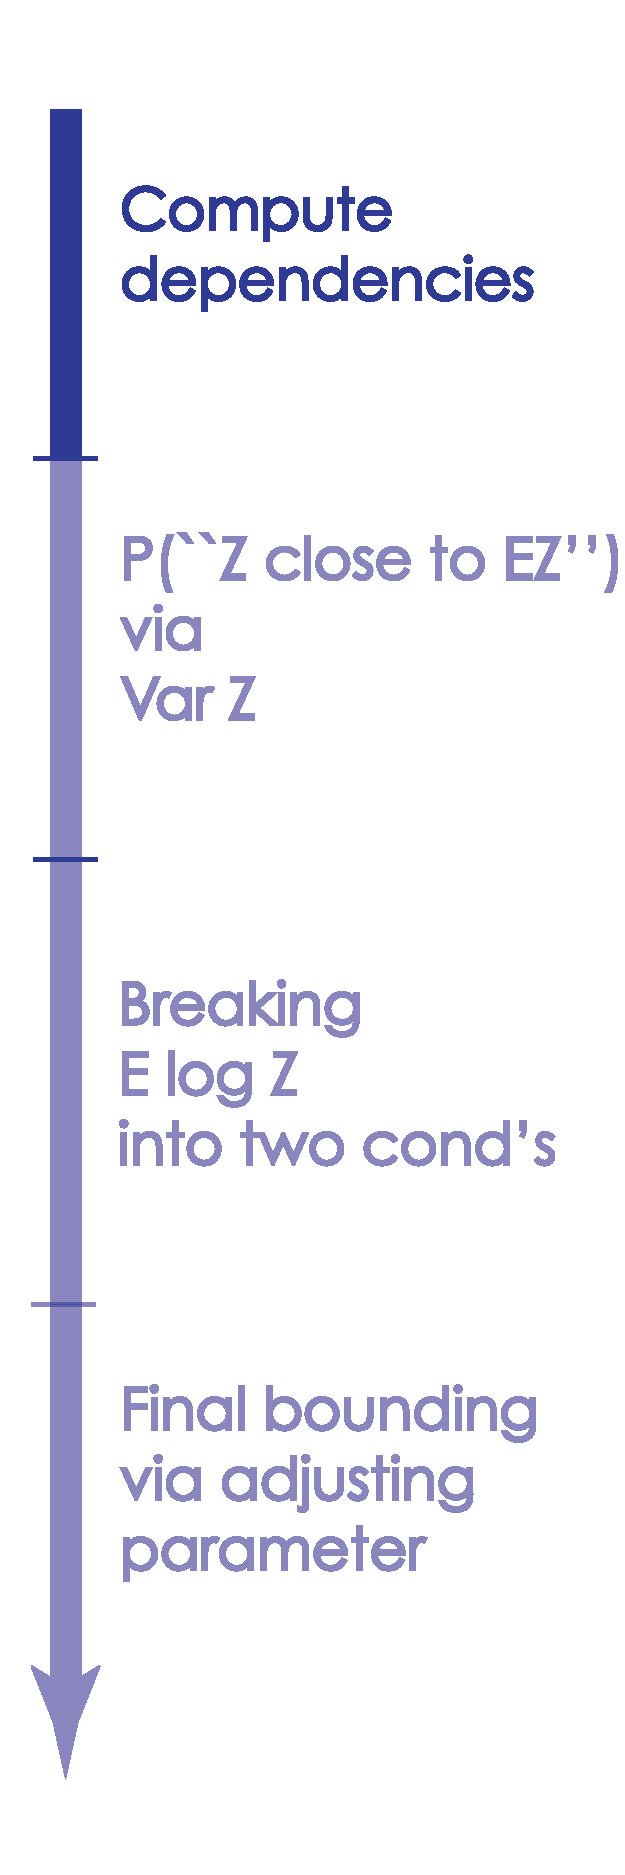
\includegraphics[scale=.23]{Proof-1.pdf}}
%   \only<2>{
%   \hfill 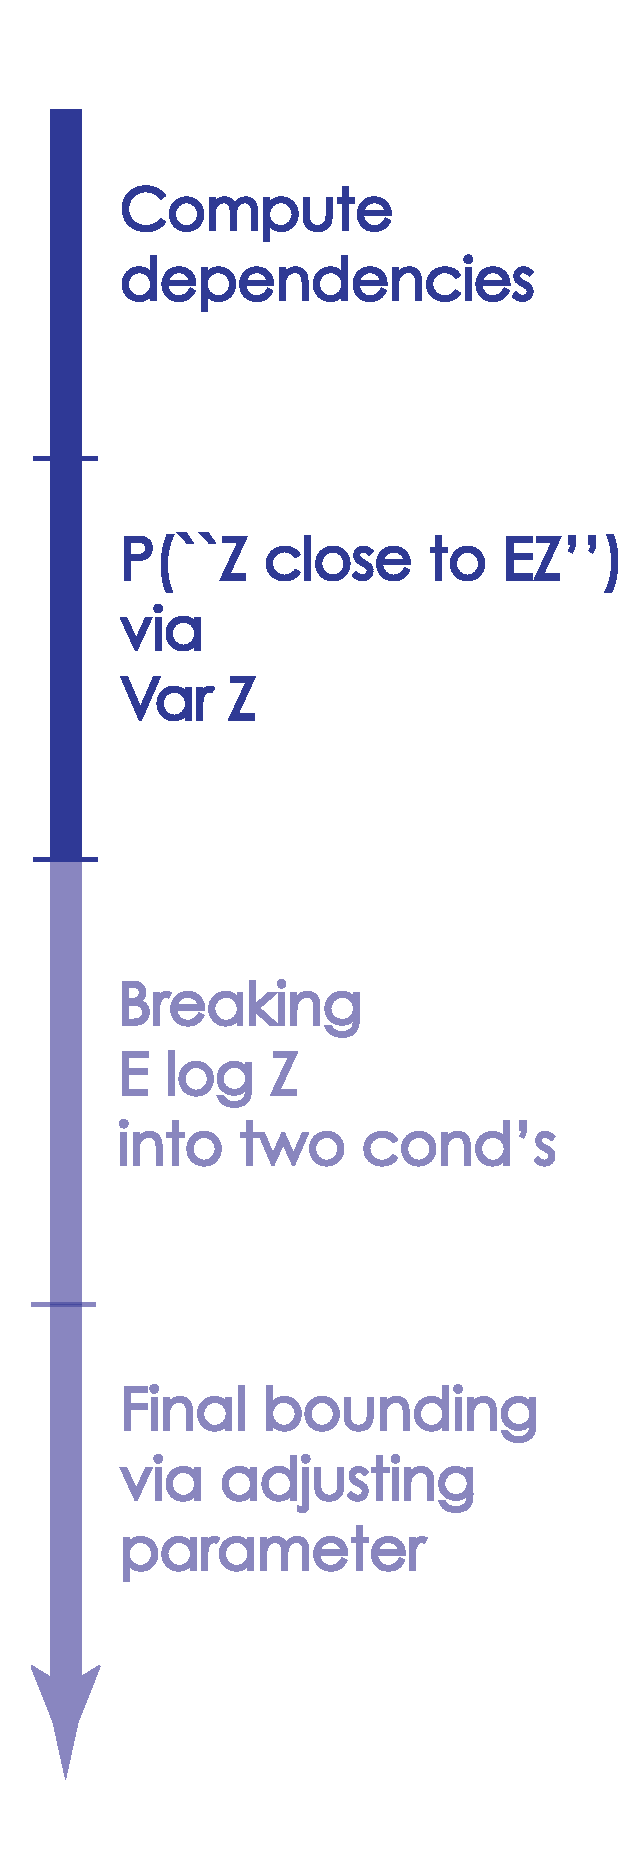
\includegraphics[scale=.23]{Proof-2.pdf}}
%   \only<3>{
%   \hfill 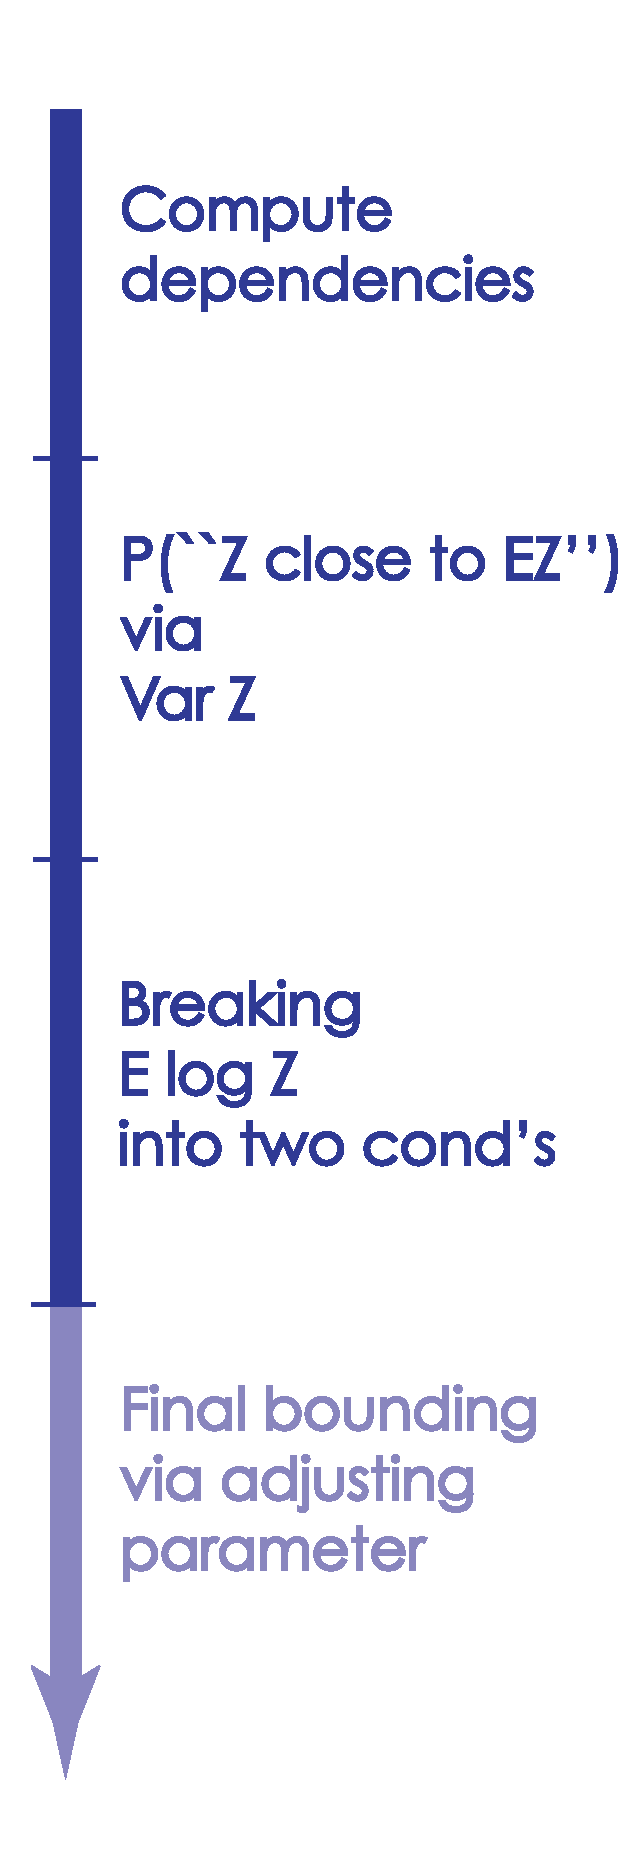
\includegraphics[scale=.23]{Proof-3.pdf}}
%   \only<4>{
%   \hfill 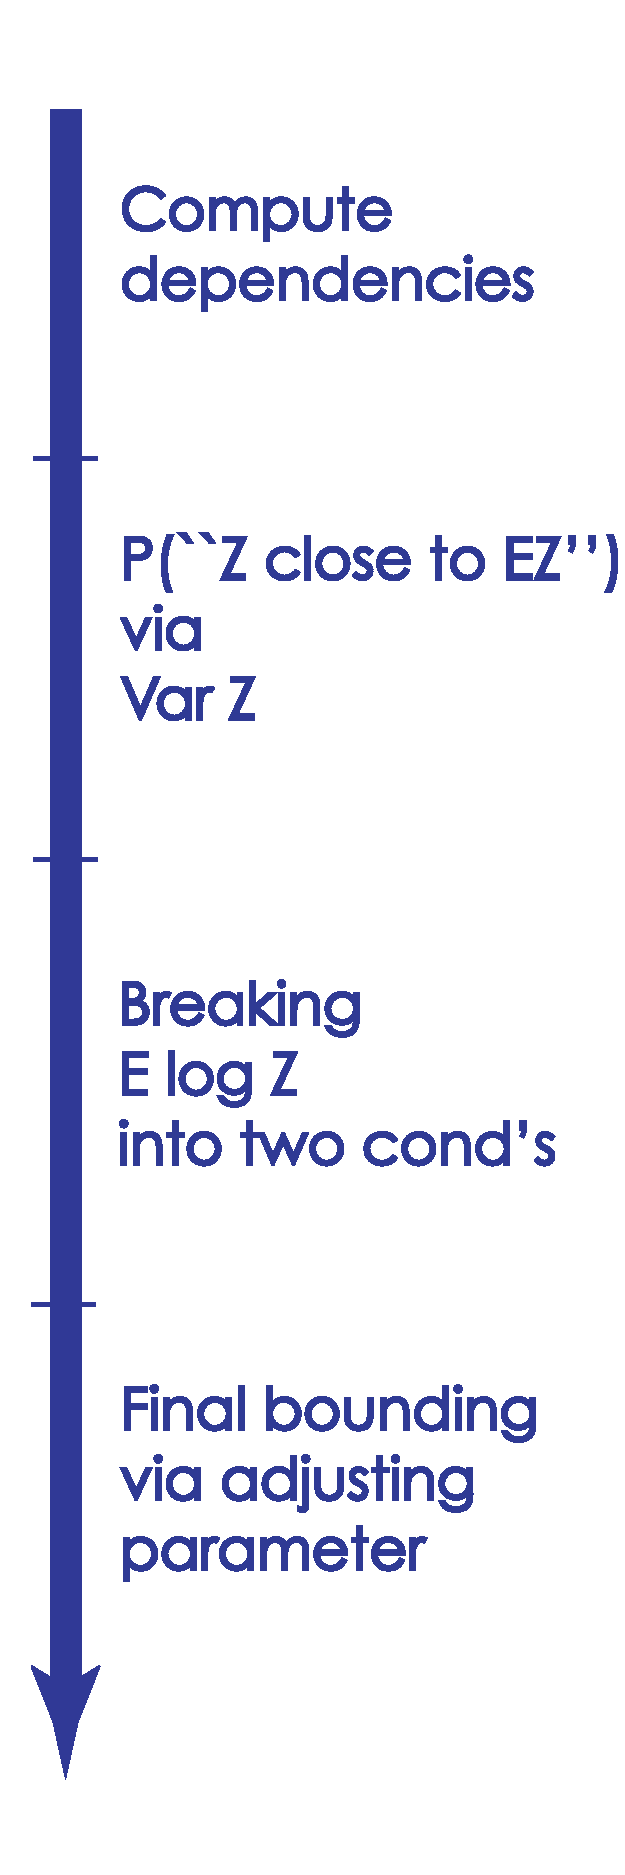
\includegraphics[scale=.23]{Proof-4.pdf}}

%   \end{column}
%   \end{columns}
% \end{frame}
% \begin{frame}{Proof Outline}
% \begin{center}
%   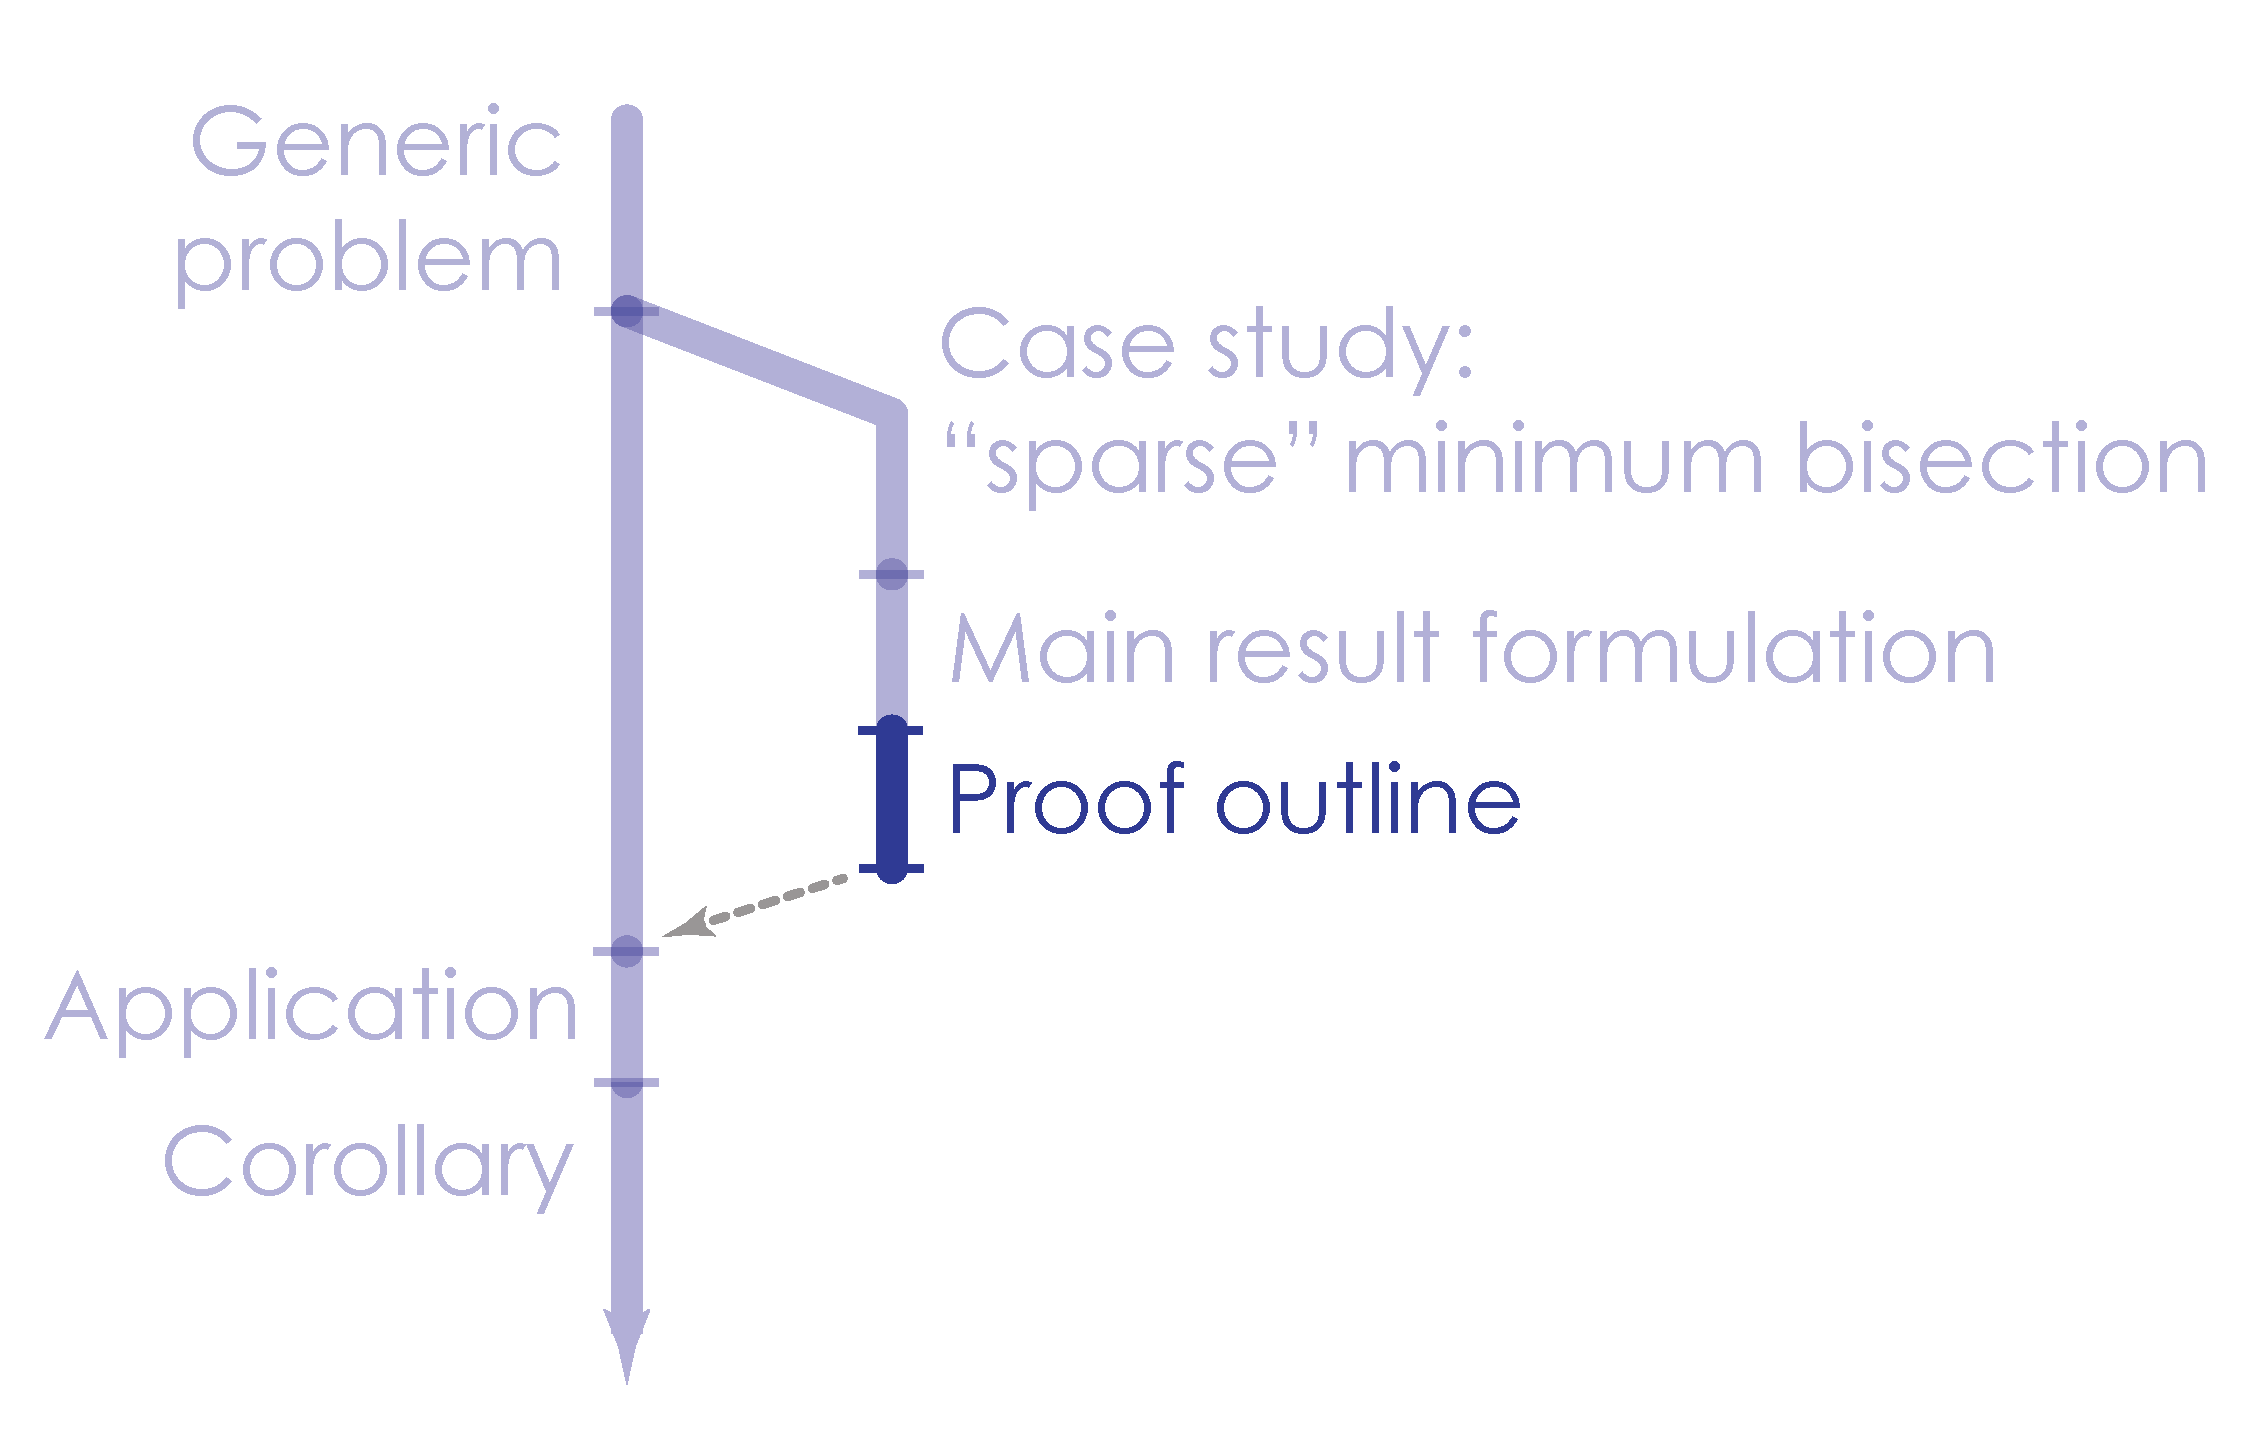
\includegraphics[scale=.27]{ProofOutline.pdf} 
% \end{center}

% \end{frame}

{\setroadmapfootline \begin{frame}[noframenumbering]{Tuning $\beta$ for Approximation}
\centering
\includegraphics[width=\textwidth]{roadmap_after_main_result} 
\end{frame}}

\begin{frame}{Role of $\beta$ in Posterior Distribution}
\begin{itemize}
  \item<+-> Recall our approach:

  \begin{center}
    \hspace{-8mm}\includegraphics[scale=.4]{posterior-distribution-explanation} 
  \end{center}
\end{itemize}

\uncover<2->{
\begin{example}[Gibbs Posterior]
  \begin{columns}[T]
    \begin{column}{0.4\textwidth}
      %\resizebox{\linewidth}{!}{%
\begin{tikzpicture}
	\begin{axis}[
	width=1.3\textwidth,
	xticklabels={,,},
	yticklabels={,,},
	ymin=0,
    	ymax=1.5,
	xlabel=\tiny{solutions $c$},
	ylabel=\tiny{$p_\beta(c | X)$},
	xticklabel style={inner sep=0pt},
	yticklabel style={inner sep=0pt}
	]
	\only<1>{\addplot[
	   red,
	   very thick,
	   domain=-2:2,
	   samples=201,
	]
	   {exp(-(x)^2 / (2*0.1)) / (sqrt(0.1 * 2*pi))};}
	   
	%%
	\only<2>{\addplot[
	   red,
	   very thick,
	   domain=-2:2,
	   samples=201,
	]
	   {exp(-(x)^2 / (2*0.5)) / (sqrt(0.5 * 2*pi))};}
	%%
	\only<3>{\addplot[
	   red,
	   very thick,
	   domain=-2:2,
	   samples=201,
	]
	   {exp(-(x)^2 / (2*1)) / (sqrt(1 * 2*pi))};}
	\only<1->{%
	\draw[densely dashed] ({axis cs:0,0}|-{rel axis cs:0,0}) -- ({axis cs:0,0}|-{rel axis cs:0,1}) node[midway, above, sloped, yshift=-.1cm] {\tiny{optimal $c^\bot$}};}%
	  %%
	\only<4->{\addplot[
	   red,
	   very thick,
	   domain=-2:2,
	   samples=201,
	]
	   {exp(-(x)^2 / (2* 2)) / (sqrt(2 * 2 * pi))};}
	\end{axis}
	\end{tikzpicture}%
%}
    \end{column}
    \begin{column}{0.6\textwidth}
      \[
        p_\beta(c | X) = \frac{\exp\bigl(-\beta R(c, X)\bigr)}{ \sum_{\tilde{c}\in \C} \exp\bigl(-\beta R(\tilde{c}, X)\bigr) }
      \]
      \uncover<2-4>{Picture: $\beta$ is \textbf{decreasing}.}
    \end{column}
  \end{columns} 
\end{example} 
}
\end{frame}

\begin{frame}{Tuning the $\beta$-Regularization}
\begin{itemize}
  \item Recall our approach:
  \begin{center}
    \hspace{-8mm}\includegraphics[scale=.4]{posterior-distribution-explanation} 
  \end{center}
  \vspace{.3cm}

  \item \textbf{Q:} how to tune $\beta$ (the \textbf{regularizer})? \\[.3cm] \textbf{A:} maximize \textbf{expected
  log-posterior agreement} (eLPA) [1]:
  \[
    \beta^* = \arg \max_\beta \underbrace{\Expct_{X',X''} \Bigl[
      \log \sum_c p_\beta(c|X') p_\beta(c|X'') 
    \Bigr]}_{\mathrm{eLPA}(\beta)}
  \]
\end{itemize}

{
  \setstretch{0.7}
  \textcolor{gray!60}{
    \scriptsize [1] Buhmann et al. (under review), 
    \textit{Posterior Agreement for Parameter-Rich Optimization Problems in the Asymptotic Limit}, J. Theor. Comp. Sc. 
  }\par
}

\end{frame}

\begin{frame}{eLPA($\beta$): Intuition}
  
  \begin{itemize}
    \item It stabilizes solution output:
  \end{itemize}

  \vspace{-3mm}
  \centering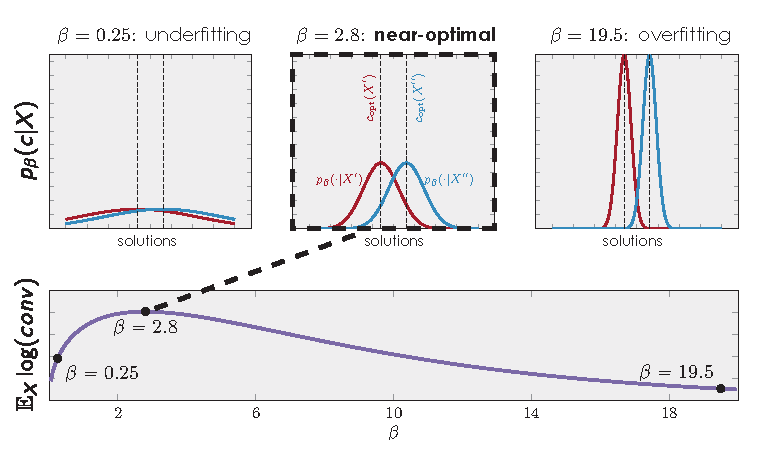
\includegraphics[scale=.85]{expected-conv-intuition.pdf}

  \begin{itemize}
    \item eLPA $\approx$ cross entropy;
  \end{itemize}
\end{frame}

{\setroadmapfootline \begin{frame}[noframenumbering]{Computing and Maximizing eLPA($\beta$)}
\centering
\includegraphics[width=\textwidth]{roadmap_after_elpa_motivation} 
\end{frame}}


\begin{frame}{Theorem: eLPA($\beta$) Asymptotics}
\only<1>{
  \begin{itemize}
  \item eLPA can be rewritten:
    \begin{align*}
      \Expct_{X', X''} &\log \sum_c p_\beta(c|X') p_\beta(c|X'') = \\
        &\underbrace{\Expct_{X', X''} \log Z(\beta, X' + X'')}_{\text{Thm from above}} \\
        &- \underbrace{\Expct_{X'} \log Z(\beta, X')}_{\text{Thm from above}} \\
        &- \underbrace{\Expct_{X''} \log Z(\beta, X'')}_{\text{Thm from above}}
    \end{align*}

  % \item<+-> Thus possible to analytically compute score:\\[2mm]
  %   \centering
  %   \hspace*{-15 mm}\includegraphics[width=1.10\textwidth]{gc_theor_beta_up-to-100_v1.eps}
  \end{itemize}
}

\only<2>{
\begin{block}{\rule[-0.6ex]{0pt}{2.5ex}Theorem: eLPA}
  \begin{itemize} 
    \item Previous setting and additive $\tilde\sigma$-noise on edges; \\
    \item Let $\gamma
  = \tilde\sigma/\sigma$ be \textbf{noise-to-signal ratio}.
  \end{itemize}
  Then, eLPA satisfies

  \begin{center}
    \includegraphics[width=.4\textwidth]{elpa_1.png}\\
    \includegraphics[width=.9\textwidth]{elpa_2.png}
  \end{center}

\end{block}
}

\only<3>{
\begin{itemize}
\item Plot: ePLA has a clear maximum:\\[2mm]
  {
    \centering
    \hspace*{-15 mm}\includegraphics[width=1.10\textwidth]{gc_theor_beta_up-to-100_v1.eps}
  }
\item 
  \begin{block}{\rule[-0.6ex]{0pt}{2.5ex}Theorem: Optimal eLPA-temperature}
    Optimal eLPA-temperature is provided by:
    \[
      \hat{\beta}^*_{\mathrm{eLPA}} 
        := \arg \max_{\hat \beta} \mathrm{eLPA(\beta)}
        = \frac{\sqrt{2 + \gamma^2}}{\sigma(1+\gamma^2)}.
    \]
  \end{block}
\end{itemize}
}

\end{frame}

{\setroadmapfootline \begin{frame}[noframenumbering]{Expected Gibbs Risk Minimization}
\centering
\includegraphics[width=\textwidth]{roadmap_after_elpa_result} 
\end{frame}}


\begin{frame}{Minimizing Expected Gibbs Risk}
  \begin{itemize}
    \item<+-> Since the expected Gibbs risk equals
    \[
      \Expct_{p_\beta(c|X), X}[R(c,X)] = - \frac{\partial}{\partial \beta} \Expct_X \log Z(\beta, X)
    \]
    \item<+-> We can apply the same theorem to directly minimize it. 
    \begin{block}{\rule[-0.6ex]{0pt}{2.5ex}Theorem: Optimal Gibbs Risk-Temperature}
      \[
        \hat{\beta}^*_{\mathrm{GR}} 
          := \arg \min_{\hat \beta} \Expct_{p_\beta(c|X)}[R(c,X)] 
          = \frac{\sqrt{2 +  2\gamma^2}}{\sigma(1+\gamma^2)}.
      \]
    \end{block}
  \end{itemize}
\end{frame}

\begin{frame}{Discrepancy: $\hat{\beta}^*_{\mathrm{eLPA}}$ and $\hat{\beta}^*_{\mathrm{GR}}$}
  \begin{itemize}
    \item The eLPA gives
    \[
      \hat{\beta}^*_{\mathrm{eLPA}} = \frac{\sqrt{2 + \gamma^2}}{\sigma(1+\gamma^2)}.
    \]
    \item The expected Gibbs risk is minimized at
    \[
      \hat{\beta}^*_{\mathrm{GR}} = \frac{\sqrt{2 + {\color{red} \boldsymbol 2}\gamma^2}}{\sigma(1+\gamma^2)}.
    \]
    \item They related only via signal-to-noise ratio:
    \[
      \frac{\hat{\beta}^*_{\mathrm{GR}}}{\hat{\beta}^*_{\mathrm{eLPA}}} 
        = \sqrt{1 + \frac{\gamma^2}{2+\gamma^2} }.
    \]

  \end{itemize}
\end{frame}

{\setroadmapfootline \begin{frame}[noframenumbering]{Finally}
\centering
\includegraphics[width=\textwidth]{roadmap_after_risk} 
\end{frame}}

{\setroadmapfootline \begin{frame}[noframenumbering]{Overview and Outlook}
\centering
\includegraphics[width=\textwidth]{roadmap_conclusion} 
\end{frame}}

{\setroadmapfootline
\begin{frame}[noframenumbering]{More for Discussion: See Appendix}
\centering
\vspace*{3pt}
\hspace*{-.4cm}\includegraphics[width=1.07\textwidth]{roadmap_larger_map} 
\end{frame}}

{\setroadmapfootline
\begin{frame}[noframenumbering]{List of Publications}

\scriptsize

    --- \textbf{Gronskiy, A.}, Buhmann, J. M., 2014. \textit{How informative are minimum
    spanning tree algorithms?} \\
    ISIT 2014
    \medskip

    --- Buhmann, J. M., \textbf{Gronskiy, A.}, Szpankowski, W., 2014. \textit{Free energy rates
    for a class of very noisy optimization problems.} \\
    AofA 2014
    \medskip

    --- Buhmann, J. M., Dumazert, J., \textbf{Gronskiy, A.}, Szpankowski, W., 2017. \textit{Phase
    transitions in parameter rich optimization problems.} \\
    SODA-ANALCO
    2017
    \medskip

    --- Buhmann, J., \textbf{Gronskiy, A.}, Mihal\'ak, M., Pr\"oger, T.,
    \v{S}r\'amek, R., Widmayer, P., 2017. \textit{Robust optimization in the presence of
    uncertainty: A generic approach.} \\
    J. of Comp. Sci. and Systems
    \medskip

    --- [under rev.] \textbf{Gronskiy, A.}, Buhmann, J. M., Szpankowski, W., 2018. \textit{Free Energy Asymptotics
    for Problems with Weak Solution Dependencies.} \\
    ISIT 2018
    \medskip

    --- [under rev.] Buhmann, J. M., Dumazert, J., \textbf{Gronskiy, A.}, Szpankowski, W., 2018.
    \textit{Posterior Agreement for Large Parameter-Rich Optimization Problems.} \\
    J. of Theor Comp. Sci.
\end{frame}}

\begin{frame}{Thanks for your attention!}
  
  \centering
  \includegraphics[height=2.5cm]{jbuhmann.jpeg} \hspace{3pt}
  \includegraphics[height=2.5cm]{widmayer.jpeg} \hspace{3pt}
  \includegraphics[height=2.5cm]{szpan.jpg} \\[5pt]

  \includegraphics[height=1.9cm]{proeger.jpg} \hspace{1pt}
  \includegraphics[height=1.9cm]{dumazert.jpg} \hspace{1pt}
  \includegraphics[height=1.9cm]{bian.jpg} \hspace{1pt}
  \includegraphics[height=1.9cm]{sramek.jpg} \hspace{1pt}
  \includegraphics[height=1.9cm]{mihalak.jpg} \hspace{1pt}
  \includegraphics[height=1.9cm]{klute.jpg} \hspace{1pt}
  \includegraphics[height=1.9cm]{berger.jpg} \\[5pt]

  \includegraphics[width=\textwidth]{institute.jpg}\\  
\end{frame}

% \begin{frame}{Phase Transition Intuition}
% \begin{itemize}
%   \item<+-> In the high-temperature regime $\hat \beta< \frac{\sqrt{2}}{\sigma}$ the solutions (configurations) are obtaining the same Gibbs weight, which results in constant leading term;
%   \item<+-> However, a low-temperature regime $\hat \beta \ge \frac{\sqrt{2}}{\sigma}$ shrinks the set of more preferred solutions, making their influence (and thus the influence of noise variance $\sigma$) more crucial, which results in the $\hat \beta \sigma \sqrt{2}$ leading term;
%   \item<+-> Note that the terms \emph{high-} and \emph{low-} refer to the \emph{normalized} temperature regimes. In overall, due to the normalization $\beta=\hat \beta \sqrt{\log m/N}$, the asymptotic analysis refers to $\beta \to 0$.
% \end{itemize}
% \end{frame}

% \begin{frame}{Approximation for Partition Function}

% % \begin{theorem} 
% %   Let $D := |c \cap c'|$, where $c, c' \in \C_n$ are chosen uniformly
% %   at random. Than, provided that $\beta \E_D[D] = o(1)$ (in the limit
% %   $n \to \infty$), the following convergence holds
% % \[
% %   Z(\beta, X) / \E_X[Z(\beta, X)] \xrightarrow{\mathbb P} 1
% % \]
% % \end{theorem}

% This (rather technical) result implies 
% \[
%   \log Z(\beta, X) \xrightarrow{\mathbb P} \log \E_X[Z(\beta, X)]
% \]
% in \alert{high-temperature} limit: not the most interesting case!
% \end{frame}

% \begin{frame}{Example: Quadratic Assignment Problem}
%   Two $n \times n$ matrices: weight matrix $V$ and the distance matrix
%   $H$.  The solution set is the set of all the $n$-element
%   permutations $S_n$. The objective function is
%   \[
%   R^{\text{\tiny QAP}}\bigl(\pi, (V,H)\bigr) = \sum_{i,j =1}^n V(i,j) \cdot
%   H\bigl(\pi(i), \pi(j)\bigr), \quad \pi \in S_n.
%   \]
%   Thus, in our notation, $\mathcal{C} = S_n$, $N = n^2$ and $m = n!$,
%   which meets the condition
%   \[
%   \log m = o(N),
%   \]
%   thus making it possible to compute $\E \log Z$ asymptotically for
%   high-temperature regimes. 
% \end{frame}

% \begin{frame}{Example: Gibbs Distribution Inference}
%   \onslide<+->{\begin{align*}
%           \E_{X', X''} [I_\beta(X', X'')] &= \E \Bigl[ \log  |\C|
%           \sum_{c \in \C} p_\beta(c | X') p_\beta(c | X'') \Bigr] \\ 
%           &= \log  |\C| + \E \Bigl[ \alert{\log Z(\beta, X', X'')} \\
%           &\phantom{= }~ - \alert{\log Z(\beta, X')} - \alert{\log
%             Z(\beta, X'')} \Bigr],
%   \end{align*}
%   where 
%   \[
%     Z(\beta, X', X'') = \log \sum_{c\in \C} \exp\bigl(-\beta R(c, X') - \beta R(c,X'')\bigr).
%   \]}
%   \onslide<+->{\begin{block}{Result}
%   The above analysis allows us to compute the posterior agreement asymptotically for discussed types of problems.
%   \end{block}}
% \end{frame}



\appendix

\setfootline{
  \textcolor{gray!60}{
    \tiny\insertshortdate \hfill \insertshortauthor \quad 
    Appendix-\insertframenumber/\inserttotalframenumber
  }
}


\begin{frame}{Appendix: Entropy and Free Energy}
\begin{align*}
  H(p_\beta) &= -\sum_{c\in \C} p_\beta(c) \log p_\beta(c) \notag \\
    &= \log Z(\beta) - \Expct_{p_\beta(c)}[R(c)] \notag \\
    &= \log Z(\beta) - \sum_{c \in \C} \frac{- \beta R(c) e^{-\beta R(c)}}{Z(\beta)} \notag \\
    &= \log Z(\beta) - \beta \, \frac{\partial}{\partial \beta} \log Z(\beta).
\end{align*}
\end{frame}

\begin{frame}{Appendix: Proof Outline -- I}
  
  \begin{columns}
  \begin{column}{0.8\textwidth}
    \begin{itemize}
      \item Introduce ``solution overlap'' $D$: average intersection of
      two bisections
      \item $D$ is key to understand \textbf{dependencies} (remember 
      we are no REM!)
    \end{itemize}
  \vspace{1em}

  \begin{block}{\rule[-0.6ex]{0pt}{2.5ex}Lemma 1}
  The following holds
  \[
      \mathbb{E}_{\text{rand choice}} D = \mathcal{O}(d^4 / n).
    \]
  % \end{lemma}
  \end{block}

  \end{column}
  \begin{column}{0.2\textwidth}
  \hfill 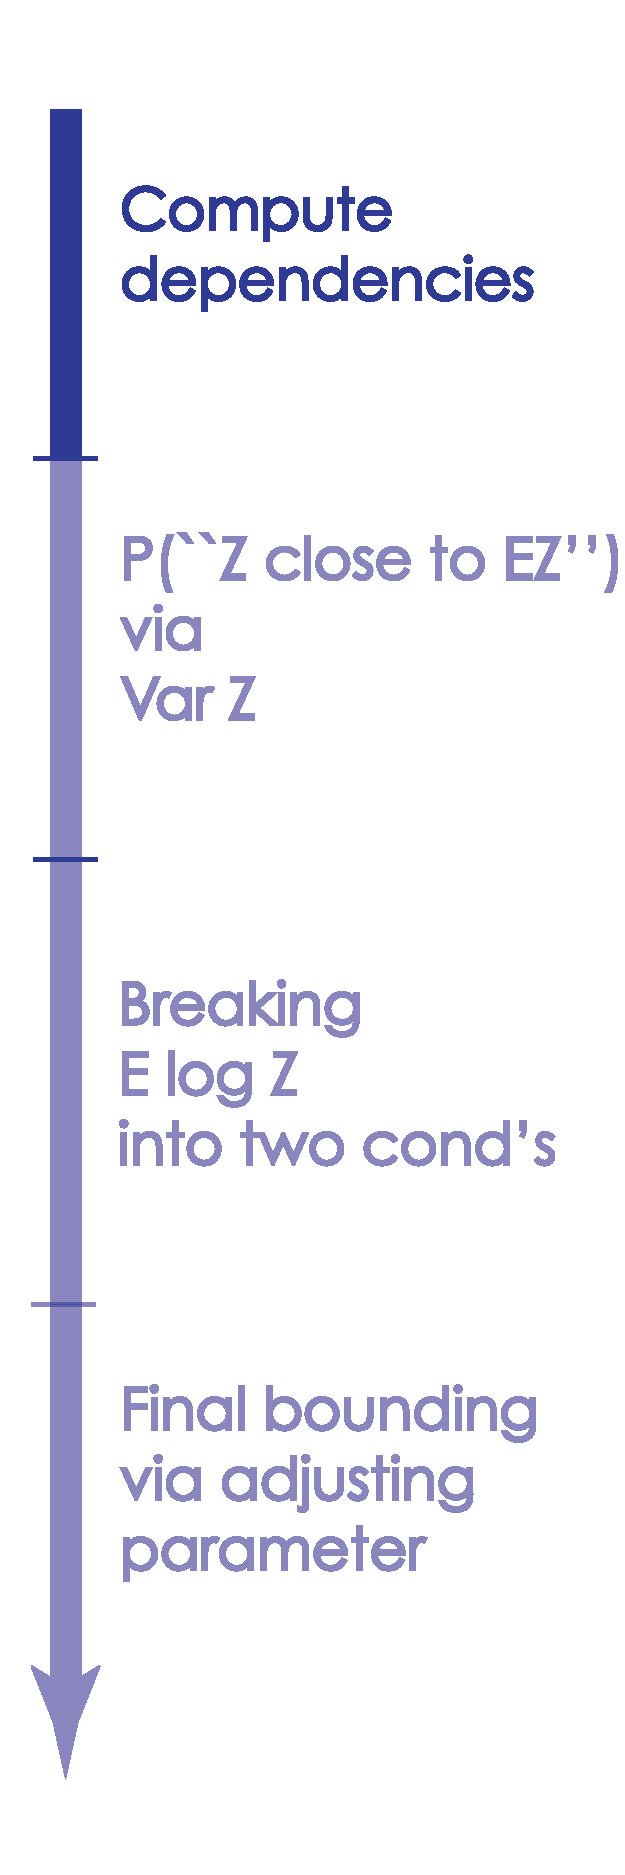
\includegraphics[scale=.23]{Proof-1.pdf}

  \end{column}
  \end{columns}

\end{frame}

\begin{frame}{Appendix: Proof Outline -- II}
  \begin{columns}
  \begin{column}{0.8\textwidth}
    \begin{itemize}
      \item Introduce event $A$: happens when $Z$ is close to $\mathbb{E}Z$, i.~e.
        $A := \{ Z \ge \epsilon \mathbb{E} Z \}$
      \item Goal is to compute $\mathbb{P}(A)$
    \end{itemize}

  \begin{block}{\rule[-0.6ex]{0pt}{2.5ex}Fact 2}
    $\mathbb{P}(A)$ can be bounded by $\Var Z$ via Chebychev.
  \end{block}

  \begin{block}{\rule[-0.6ex]{0pt}{2.5ex}Lemma 3 [Buhmann et al., 2014]}
    $\Var Z$ can be asymptotically approximated via $\mathbb{E}_{\text{rand choice}} D$:
    \[
      \Var Z \sim (\Expct Z)^2 
          \bigl( \sigma^2 \beta^2 \Expct_{\text{rand choice}} D \bigr).
    \]
  \end{block}

  \end{column}
  \begin{column}{0.2\textwidth}
  \hfill 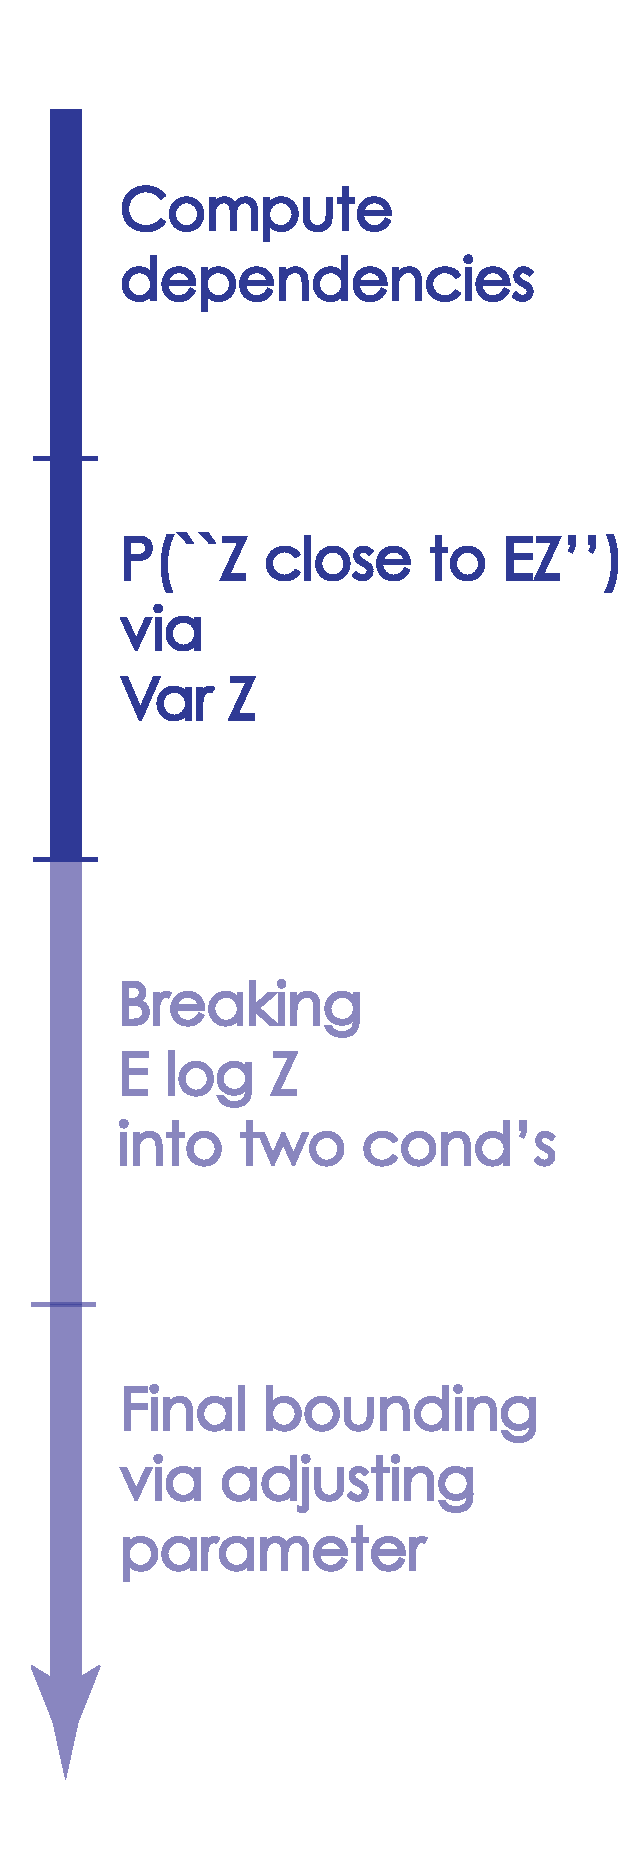
\includegraphics[scale=.23]{Proof-2.pdf}

  \end{column}
  \end{columns}
\end{frame}

\begin{frame}{Appendix: Proof Outline -- III}
  \begin{columns}
  \begin{column}{0.8\textwidth}
    \begin{itemize}
      \item Break $\Expct \log Z$ into 
      \begin{align*}
          \Expct \log Z &= \Expct [\log Z \mid A] \cdot \Prob(A) 
            + \Expct[\log Z \Ind(\bar A)] \notag \\
          &\!\!\!\!\!\!\!\!\ge (\log \Expct Z + \log \epsilon) \Prob(A) 
            + \Expct[\log Z \Ind(\bar A)]
      \end{align*}
    \end{itemize}

  \vspace{-1em}

  \begin{block}{\rule[-0.6ex]{0pt}{2.5ex}Fact 4}
  Can expand $\log \Expct Z$ via Taylor expansion (used assumptions of
  Theorem) and bound $\Prob(A)$ from previous.
  \end{block}

  \begin{block}{\rule[-0.6ex]{0pt}{2.5ex}Fact 5}
    $\Expct[\log Z \Ind(\bar A)]$: enough to bound loosely
  \end{block}

  \end{column}
  \begin{column}{0.2\textwidth}
  \hfill 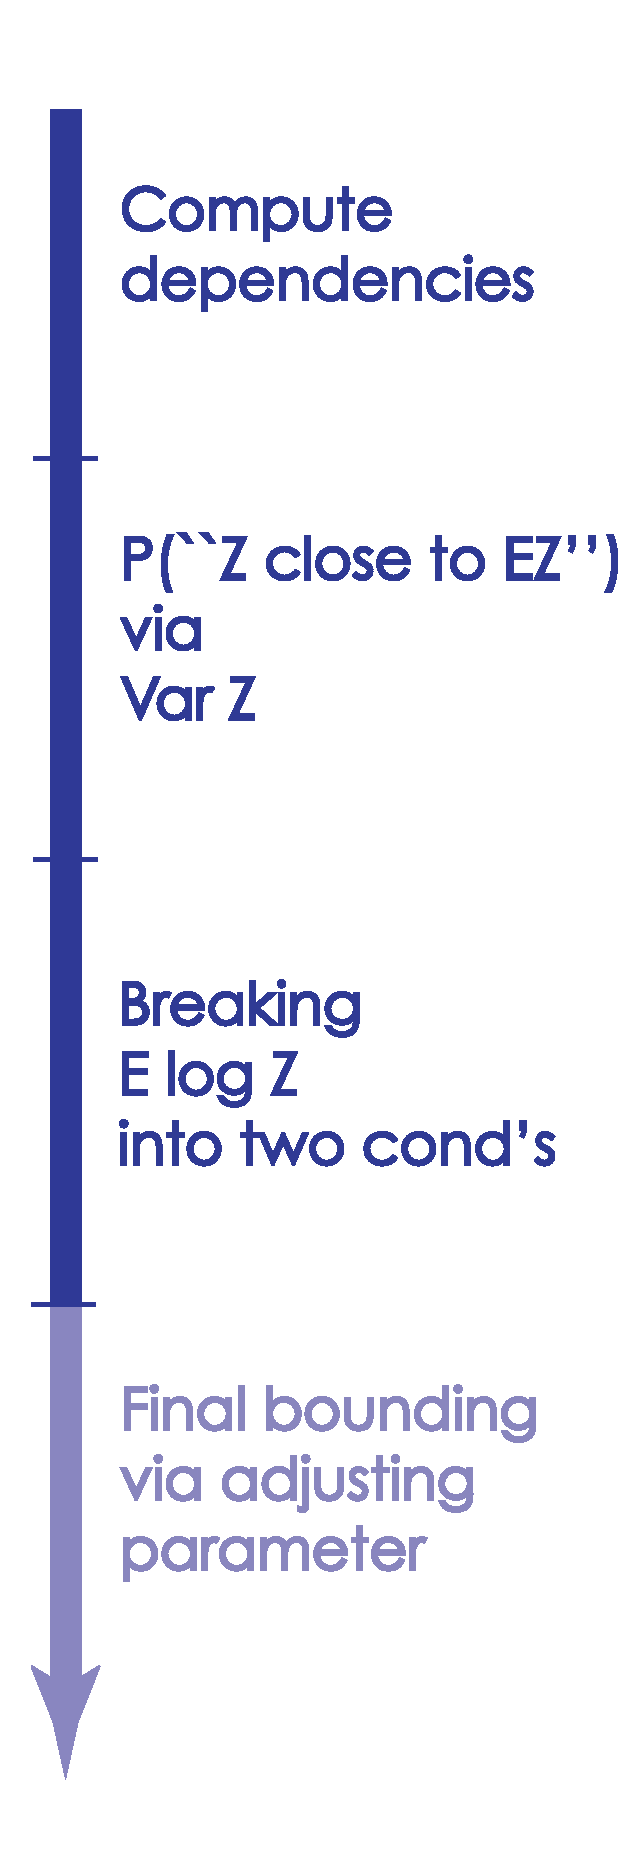
\includegraphics[scale=.23]{Proof-3.pdf}

  \end{column}
  \end{columns}
\end{frame}

\begin{frame}{Appendix: Proof Outline -- IV}
  \begin{columns}
  \begin{column}{0.8\textwidth}
    \begin{itemize}\setlength\itemsep{1em}
    \item Finally, the right choice of $\epsilon$ for two regimes of $\beta$
    gives the phase transition in \textbf{lower bound}
    
    \vspace{-1em}
    \[
      \lim_{n\to \infty} \frac{\E[\log Z] + \cdots}{\cdots} > 
      \left\{ 
        \begin{array}{ll}
          1+\frac{\hat \beta^2\sigma^2}{2}, &
          \hat \beta< \frac{\sqrt{2}}{\sigma},\\
          \hat \beta \sigma \sqrt{2}, & \hat \beta \ge \frac{\sqrt{2}}{\sigma}.
        \end{array}
      \right.
    \]
    

    \item The \textbf{same} phase transition happens for \textbf{upper
    bound},~--- easier to prove (no need to compute dependencies)

    \end{itemize}

  \end{column}
  \hspace{5.5 pt}
  \begin{column}{0.2\textwidth}
  \hfill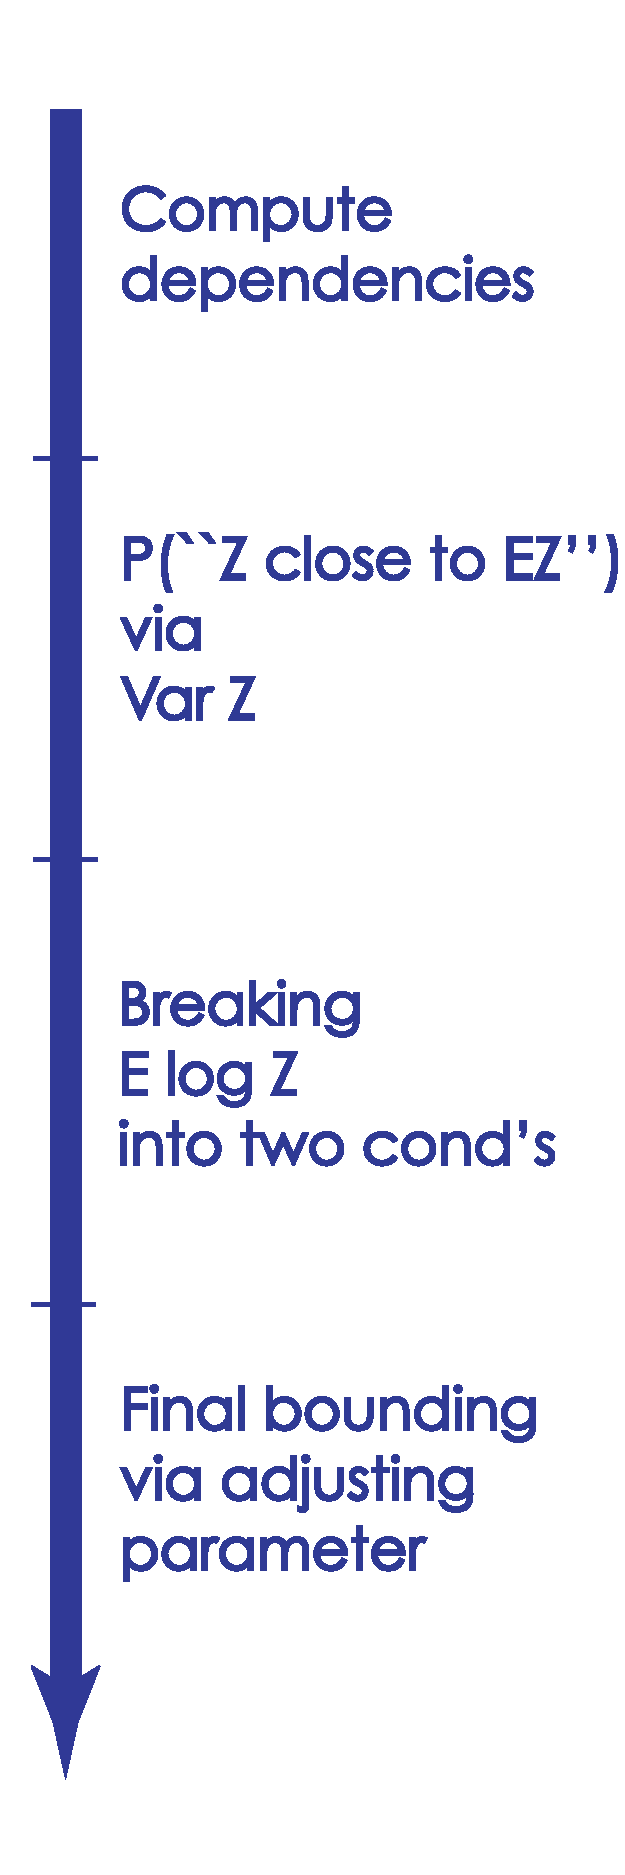
\includegraphics[scale=.23]{Proof-4.pdf}

  \end{column}
  \end{columns}
\end{frame}

% \begin{frame}{Appendix: Why Coding?}
%   \begin{tikzpicture}

% \only<1-7>{\node[color=red, align=center] at (3,5) {$X'$ defines original \\ codebook solutions $p_\beta\bigl(c | \tau(X') \bigr)$};
% \node[align=center] at (2.5, 4) {Sent $\tau_4(X')$};
% }
% \only<2-7>{\node[color=blue, align=center] at (2.5,2.5) {$X''$ defines shifted solutions \\ (how error occurs!) \\ Received $\tau_4(X'')$};}
% \only<4-7>{\node[align=center] at (2.5,1) {Decoding $\tau$: max overlap \\ (as in Hamming decoding!)};}
% \only<8->{\node[align=center] at (2.5,1) {Better rate --- less robust \\ (wrong decoding!)};}

\coordinate (x11) at (8.5,3.3);
\coordinate (x12) at (7.7,1.9);
\coordinate (x13) at (8.5,0.5);
\coordinate (x14) at (6,2);
\coordinate (x15) at (9.5,2);
\coordinate (x16) at (6.7,3.5);
\coordinate (x17) at (6.7,0.5);

\coordinate (x18) at (6.3,1.2);
\coordinate (x19) at (6.9, 1.6);
\coordinate (x110) at (6.7,2.5);
\coordinate (x111) at (7.8,2.7);
\coordinate (x112) at (8.5,2);
\coordinate (x113) at (7.6,0.9);

\coordinate (x11shift) at (0.2, 0.3);
\coordinate (x12shift) at (-0.3, 0.3);
\coordinate (x13shift) at (-0.2, 0.3);
\coordinate (x14shift) at (0.2, -0.6);
\coordinate (x15shift) at (-0.2, -0.3);
\coordinate (x16shift) at (0.3, -0.35);
\coordinate (x17shift) at (0.2, 0.3);

\foreach \x in {x11,x12,x13,x14,x15,x16,x17}
{
	\filldraw[color=red] (\x) circle (0.1cm);
	\only<1-3>{\filldraw[color=red, fill opacity=0.1] (\x) circle (0.9cm);}
}

\foreach \x in {2,3,4,5,6,7}
{
	\only<1>{\draw[->, shorten >=0.1cm, color=red] (x11) to node[pos=0.95, above, color=black] {$c(\tau_{\x})$} (x1\x);}
}
\only<1>{\draw[->, shorten >=0.1cm, color=red, ultra thick] (x11) to (x14);}

\foreach \x in {x11,x12,x13,x14,x15,x16,x17}
{
	\coordinate (2\x) at ( $(\x) + (\x shift)$ );
	\only<2-4>{\filldraw[color=blue] (2\x) circle (0.1cm);}
	\only<2-4>{\draw[->, shorten >=0.1cm, color=blue] (\x) to (2\x);}
	\only<3-3>{\filldraw[color=blue, fill opacity=0.1] (2\x) circle (0.9cm);}
}

\only<2>{\node[align=center] at (8,-1) {Noise in $X$: shifting $p_\beta(c | X)$};}

\only<4-5>{%
	\filldraw[color=red, fill opacity=0.1] (x14) circle (0.9cm);
	\filldraw[color=red, fill opacity=0.1] (x12) circle (0.9cm);
	\filldraw[color=red, fill opacity=0.1] (x17) circle (0.9cm);
	\filldraw[color=blue, fill opacity=0.3] (2x14) circle (0.9cm);
}

\only<5>{
	\filldraw[color=red, fill opacity=0.7] (x14) circle (0.9cm);
	\filldraw[color=blue] (2x14) circle (0.1cm);
	\draw[->, shorten >=0.1cm, color=blue] (x14) to (2x14);
}

\foreach \x in {x11,x12,x13,x14,x15,x16,x17, x18, x19, x110, x111, x112, x113}
{
	\only<6->\filldraw[color=red] (\x) circle (0.1cm);
	\only<6>{\filldraw[color=red, fill opacity=0.1] (\x) circle (0.5cm);}
}

\only<6->{\filldraw[color=blue] (2x14) circle (0.1cm);
\draw[->, shorten >=0.1cm, color=blue] (x14) to (2x14);}

\only<7-8>{%
	\filldraw[color=red, fill opacity=0.1] (x14) circle (0.5cm);
	\filldraw[color=red, fill opacity=0.1] (x19) circle (0.5cm);
	\filldraw[color=red, fill opacity=0.1] (x18) circle (0.5cm);
	\filldraw[color=blue, fill opacity=0.3] (2x14) circle (0.5cm);
}

\only<8>{\filldraw[color=red, fill opacity=0.7] (x18) circle (0.5cm);}

\draw[draw=none] (0,-2) -- (0,6) -- (9, 6) -- (9,-2);

\end{tikzpicture}
% \end{frame}

\begin{frame}{Intuition: Informativeness vs Robustness}
  \begin{tikzpicture}

\node[color=red] (1) at (1.5,3) {$X'$};
\node[color=blue] (2) at (1.5,2) {$X''$};
\node[color=black!60!green] (3) at (1.5,1) {$X'''$};

\coordinate (FirstCenter) at (7.4,3);
\coordinate (SecCenter) at (6.5,2);
\coordinate (ThirdCenter) at (7,1);

\draw [decorate,decoration={brace,amplitude=10pt}]
(1.2,0.9) -- (1.2,3.1) node [black,midway,xshift=-0.8cm] {$\mathbb{P}(X)$};

\draw[->,shorten >=0.3cm, color=red,thick,out=0,in=160] (1) to node [pos=0.2,fill=white] {$R(c, X')$} (FirstCenter) ;
\draw[->,shorten >=0.3cm, color=blue,thick,out=0,in=160] (2) to node [pos=0.2,fill=white] {$R(c, X'')$} (SecCenter) ;
\draw[->, shorten >=0.3cm, color=black!60!green,thick,out=0,in=160] (3) to node [pos=0.2,fill=white] {$R(c, X''')$} (ThirdCenter) ;

\draw[draw=none] (0,-2) -- (0,6) -- (10, 6) -- (10,-2);

\only<1>{%
\filldraw[color=red, fill opacity=0.2] (FirstCenter) circle (2.6);
\filldraw[color=blue, fill opacity=0.2] (SecCenter) circle (2.3cm);
\filldraw[color=black!60!green, fill opacity=0.2] (ThirdCenter) circle (2.7cm); }

\only<2>{%
\filldraw[color=red, fill opacity=0.2] (FirstCenter) circle (1.9cm);
\filldraw[color=blue, fill opacity=0.2] (SecCenter) circle (2cm);
\filldraw[color=black!60!green, fill opacity=0.2] (ThirdCenter) circle (2.2cm); }

\only<3>{%
\filldraw[color=red, fill opacity=0.2] (FirstCenter) circle (1.5cm);
\filldraw[color=blue, fill opacity=0.2] (SecCenter) circle (1.2cm);
\filldraw[color=black!60!green, fill opacity=0.2] (ThirdCenter) circle (1.4cm); }

\only<4>{%
\filldraw[color=red, fill opacity=0.2] (FirstCenter) circle (0.7cm);
\filldraw[color=blue, fill opacity=0.2] (SecCenter) circle (0.5cm);
\filldraw[color=black!60!green, fill opacity=0.2] (ThirdCenter) circle (0.6cm); }

\only<5>{%
\filldraw[color=red, fill opacity=0.2] (FirstCenter) circle (0.2cm);
\filldraw[color=blue, fill opacity=0.2] (SecCenter) circle (0.3cm);
\filldraw[color=black!60!green, fill opacity=0.2] (ThirdCenter) circle (0.25cm); }

\only<1-6>{%
\filldraw[color=red] (FirstCenter) circle (0.1cm);
\filldraw[color=blue] (SecCenter) circle (0.1cm);
\filldraw[color=black!60!green] (ThirdCenter) circle (0.1cm); }

\node[align=center] at (1,4.5) {Data \\ Inputs};
\node[align=center] at (4,4.5) {Solving \\ (Approximating)};
\node[align=center] at (8,4.5) {Optimal Solutions \\ (Approx. Sets)};
\only<2->{%
\node[align=center] at (7,-1) {Increasing $\beta$ (decreasing $\gamma$) \\
Extracts more information from input.};}
\end{tikzpicture}
\end{frame}

\begin{frame}{Appendix: Free Energy Conjecture}
  \centering
  \includegraphics[width=\textwidth]{conjecture_1.png} \\
  \includegraphics[width=.55\textwidth]{conjecture_2.png} \\
  \includegraphics[width=\textwidth]{conjecture_3.png}
\end{frame}

\begin{frame}{Appendix: Replica Trick}
  \centering
  \includegraphics[width=0.3\textwidth]{replica.png}
\end{frame}

\begin{frame}{Appendix: Various Posteriors}
  \uncover<1-4>{\begin{example}[Gibbs Posterior]
  \begin{columns}[T]
    \begin{column}{0.3\textwidth}
      %\resizebox{\linewidth}{!}{%
\begin{tikzpicture}
	\begin{axis}[
	width=1.3\textwidth,
	xticklabels={,,},
	yticklabels={,,},
	ymin=0,
    	ymax=1.5,
	xlabel=\tiny{solutions $c$},
	ylabel=\tiny{$p_\beta(c | X)$},
	xticklabel style={inner sep=0pt},
	yticklabel style={inner sep=0pt}
	]
	\only<1>{\addplot[
	   red,
	   very thick,
	   domain=-2:2,
	   samples=201,
	]
	   {exp(-(x)^2 / (2*0.1)) / (sqrt(0.1 * 2*pi))};}
	   
	%%
	\only<2>{\addplot[
	   red,
	   very thick,
	   domain=-2:2,
	   samples=201,
	]
	   {exp(-(x)^2 / (2*0.5)) / (sqrt(0.5 * 2*pi))};}
	%%
	\only<3>{\addplot[
	   red,
	   very thick,
	   domain=-2:2,
	   samples=201,
	]
	   {exp(-(x)^2 / (2*1)) / (sqrt(1 * 2*pi))};}
	\only<1->{%
	\draw[densely dashed] ({axis cs:0,0}|-{rel axis cs:0,0}) -- ({axis cs:0,0}|-{rel axis cs:0,1}) node[midway, above, sloped, yshift=-.1cm] {\tiny{optimal $c^\bot$}};}%
	  %%
	\only<4->{\addplot[
	   red,
	   very thick,
	   domain=-2:2,
	   samples=201,
	]
	   {exp(-(x)^2 / (2* 2)) / (sqrt(2 * 2 * pi))};}
	\end{axis}
	\end{tikzpicture}%
%}
    \end{column}
    \begin{column}{0.7\textwidth}
      \[
        p_\beta(c | X) = \frac{\exp\bigl(-\beta R(c, X)\bigr)}{ \sum_{\tilde{c}\in \C} \exp\bigl(-\beta R(\tilde{c}, X)\bigr) }
      \]
      \uncover<2->{Picture: $\beta$ is \textbf{decreasing}.}
    \end{column}
  \end{columns} 
  \end{example} }
  \begin{example}[Bounded-Support Uniform]
  \begin{columns}[T]
    \begin{column}{0.3\textwidth}
      %\resizebox{\linewidth}{!}{%
\begin{tikzpicture}[
    declare function={unipdf(\x,\xl,\xu)= (\x>\xl)*(\x<\xu)*1/(\xu-\xl);}
]
	\begin{axis}[
	width=1.3\textwidth,
	xticklabels={,,},
	yticklabels={,,},
	ymin=0,
    	ymax=1.5,
	xlabel=\tiny{solutions $c$},
	ylabel=\tiny{$p_\beta(c | X)$},
	xticklabel style={inner sep=0pt},
	yticklabel style={inner sep=0pt}
	]
	\only<1>{\addplot[
	   red,
	   very thick,
	   domain=-2:2,
	   samples=201,
	]
	   { unipdf(x, -.35,.35) };}
	   
	%%
	\only<2>{\addplot[
	   red,
	   very thick,
	   domain=-2:2,
	   samples=201,
	]
	   {unipdf(x, -.5,.5) };}
	%%
	\only<3>{\addplot[
	   red,
	   very thick,
	   domain=-2:2,
	   samples=201,
	]
	   {unipdf(x, -1,1) };}
	\only<1->{%
	\draw[densely dashed] ({axis cs:0,0}|-{rel axis cs:0,0}) -- ({axis cs:0,0}|-{rel axis cs:0,1}) node[midway, above, sloped, yshift=-.1cm] {\tiny{optimal $c^\bot$}};}%
	  %%
	\only<4->{\addplot[
	   red,
	   very thick,
	   domain=-2:2,
	   samples=201,
	]
	   {unipdf(x, -1.5,1.5) };}
	\end{axis}
	\end{tikzpicture}%
%}
    \end{column}
    \begin{column}{0.7\textwidth}
      \[
        p_\beta(c | X) = \mathrm{Uniform}\bigl( C_\gamma(X) \bigr)
      \]
      where $C_\gamma$ is \textbf{$\gamma$-approximation set}:
      \[
        C_\gamma( X ) := \bigl\{ c \in \C \bigm| R( c, X ) - R( c^\bot, X ) \le \gamma \bigr\}.
      \]
      \only<1-4>{\uncover<2-4>{Picture: $\gamma$ is \textbf{increasing}.}}%
    \end{column}
  \end{columns}
  \end{example}
\end{frame}

\begin{frame}{Appendix: Shannon Coding -- I}
  \centering
  \includegraphics[width=\textwidth]{shannon_coding_1.png}
\end{frame}

\begin{frame}{Appendix: Shannon Coding -- II}
  \centering
  \includegraphics[width=\textwidth]{shannon_coding_2.png}
\end{frame}

\begin{frame}{Appendix: Coding Capacity -- I}
  \centering
  \includegraphics[width=.7\textwidth]{asc_decoding_scheme.png}
\end{frame}

\begin{frame}{Appendix: Coding Capacity -- II}
  \centering
  \includegraphics[width=.7\textwidth]{asc_decoding_scheme_2.png}
\end{frame}

\begin{frame}{Appendix: ASC Derivation -- I}
  \centering
  \includegraphics[width=\textwidth]{asc_derivation_1.png}\\
  \includegraphics[width=\textwidth]{asc_derivation_2.png}
\end{frame}

\begin{frame}{Appendix: ASC Derivation -- II}
  \centering
  \includegraphics[width=\textwidth]{asc_derivation_3.png}
\end{frame}

\begin{frame}{Appendix: Theorem eLPA Full}
  \begin{block}{\rule[-0.6ex]{0pt}{2.5ex}Theorem: eLPA}
  As previously, edge weights mutually independent
  within any given solution; have mean $\mu$ and variance $\sigma^2$. Assume
  then additive noise $\delta X'$, $\delta X''$ with mean $0$, and variance
  $\tilde{\sigma}^2$, all the sets of the same size. Let $\gamma
  = \tilde\sigma/\sigma$ be noise-to-signal ratio. Then, eLPA satisfies

  \centering
  \includegraphics[width=.4\textwidth]{elpa_1.png}\\
  \includegraphics[width=.9\textwidth]{elpa_2.png}
  \end{block}
\end{frame}

\begin{frame}{Appendix: $\gamma$-Similarity Approach}
  \centering
  \includegraphics[width=.8\textwidth]{proof-of-concept.png}
\end{frame}

\begin{frame}{Appendix: Gibbs Similarity Approach}
  \centering
  \includegraphics[width=.8\textwidth]{gibbs-proof-of-concept.png}
\end{frame}

\begin{frame}{Appendix: Estimate of Similarity -- I}
  \centering
  \includegraphics[width=\textwidth]{theor-sim.png}
\end{frame}

\begin{frame}{Appendix: Estimate of Similarity -- II}
  \centering
  \includegraphics[width=\textwidth]{annealed-sim.png}
\end{frame}

\begin{frame}{Appendix: Algorithmic $t$-eLPA}
  \centering
  \includegraphics[width=\textwidth]{algorithmic-elpa.png}
\end{frame}

\begin{frame}{Appendix: MST -- Maximum $t$-eLPA}
  \centering
  \includegraphics[width=.45\textwidth]{mst-noise.png}
  \includegraphics[width=.45\textwidth]{mst-loc-err.png}
\end{frame}

\begin{frame}{Appendix: Algorithmic $t$-eLPA}
  \centering
  \includegraphics[width=.8\textwidth]{mst-elpa.png}
\end{frame}

\end{document}
